\chapter[The post-predicate position in Kurmanji in contact]{The post-predicate position in Kurmanji in contact with German and/or Turkish}\label{chap:key:6}

This chapter investigates whether there are changes in word order in Kurmanji varieties, specifically focusing on the post-predicate domain. Unlike Turkish, Kurmanji remains an underexplored heritage language, particularly in the German context. Despite being spoken by a significant number of individuals, there is a scarcity of studies examining Kurmanji, aside from those mentioned in \sectref{sec:key:2.2}. This study aims to contribute to filling this research gap.

In contrast, the Turkish context has garnered more interest in Kurmanji among researchers, particularly regarding the post-predicate domain. However, most studies have focused on speakers from villages where the majority of residents speak Kurmanji (\citealt{Dorleijn1996, Dorleijn2006}, \citealt{Haig2014}, \citealt{Haig2018, Gundogdu2019}). This study, on the other hand, centers on young adults who are Kurmanji-Turkish bilinguals living in Ankara, an urban city with a Turkish-dominant environment, and presents data from both of their languages.

Unlike Turkish, the impact of many factors on potential language change cannot be systematically investigated in Kurmanji. A major challenge lies in identifying the source of such changes—whether they are contact-induced or internally motivated. This difficulty stems largely from the scarcity of monolingual Kurmanji speakers, as the vast majority are bilingual or multilingual. Moreover, they often show stronger dominance in the majority language of their respective countries, such as Turkish, Persian, Arabic, or other contact languages (\citealt{BrizicnodateEtAl}).

Secondly, it is difficult to assess the impact of the societal status of Kurmanji. This study investigates two speaker groups: Kurmanji-Turkish bilinguals in Turkey and Kurmanji-Turkish-German trilinguals in Germany. In both cases, Kurmanji is considered a heritage language, according to the definition provided in Chapter 1. Its use is predominantly confined to informal settings, primarily within the home and among family members in both countries.

Furthermore, although Kurmanji is studied in two countries with different majority languages, Turkish serves as the contact language for both groups. However, Turkish holds different societal statuses in each country: it is a majority language in Turkey and a heritage language in Germany. Consequently, since the dominant language typically exerts a greater influence on the minority language in contact situations, a stronger impact of Turkish on Kurmanji is anticipated in Turkey compared to its influence on Kurmanji in Germany.

Moreover, the two language contexts differ from each other in terms of the intensity of contact, which is determined by the length of contact and the number of speakers in the community. Speakers of Turkic languages have likely been in contact with Kurdish speakers for over a thousand years \citep{Haig2023}. Contact between Turkish and Kurmanji predates the Ottoman Empire and intensified following the establishment of the Turkish Republic (\citealt{Yagmur2001}). Secondly, the number of individuals of Kurdish origin in Turkey is estimated at 20 million people (\citealt{Kurdish2017}). On the other hand, the contact between Kurmanji and German in Germany started in the second half of the 20\textsuperscript{th} century with the arrival of guest workers to Germany, and the number of Kurdish people in Germany is estimated at 1,300,000 (\citealt{GhaderiAlmstadt2023}). It is however unclear how many of them identify themselves as Kurds and what language(s) they speak at home.

Finally, similar to Turkish, an important factor investigated in this study is register. Unlike Turkish, the use of the post-predicate position in Kurmanji is determined by predicate semantics and is not expected to be sensitive to communicative situations. However, several reasons warrant an examination of the impact of register. First, to date, no research has explored the influence of formality and mode on word order in Kurmanji in contact with Turkish. Additionally, studies by \citet{Frommer1981} and \citet{Haig_post-predicate_EtAl2024-1} have demonstrated the effects of formality and mode on word order in Persian, a language that shares syntactic features with other Western Iranian languages, including Kurmanji. Second, the use of the post-predicate position is closely linked to formality and mode in Turkish, which serves as the contact language for both groups of Kurmanji speakers in this study. Finally, as a heritage language, Kurmanji is typically not used in formal situations, particularly when interacting with government entities, such as the police. Nonetheless, since speakers are likely aware of the effects of formality and mode on language use in the majority language, it is intriguing to explore whether they develop novel strategies in their heritage language to conform to the linguistic conventions of specific communicative situations.

In conclusion, Kurmanji is different from the heritage languages commonly studied in heritage language research. It does not have a monolingual variety and does not function as a majority language, meaning that Kurmanji speakers in both Turkey and Germany are not exposed to the various registers typically found in other languages. While this study acknowledges that many factors present in Turkish cannot be explored in the case of Kurmanji, it nonetheless establishes a foundation for future research on Kurmanji as a heritage language.

This chapter is structured as follows. First, it presents the frequency of post-predicate constituents in Kurmanji in general (\sectref{sec:key:6.1}). Next, it analyzes the use of these constituents across different communicative situations (\sectref{sec:key:6.2}). Since the post-predicate position is reserved for certain types of constituents, in \sectref{sec:key:6.3}. the chapter focuses on two main categories: goals of motion and addressees of verbs of speech. It pays particular attention to how these constituents are flagged while also considering the effect of informality and mode, and information structure on their placement. Finally, the chapter explores other (non-goal) constituents that occur in the post-predicate position. It examines their weight, type, and semantic roles, as well as their usage across various communicative contexts.

\section{Frequency distribution of post-predicate constituents in heritage Kurmanji}\label{sec:key:6.1}

The analysis begins with an overview of the frequency distribution of post-predicate constituents in Kurmanji in Turkey and Germany. It includes all instances of post-predicate position use without distinguishing between communicative situations, resulting in four data points for each speaker.

\begin{figure}
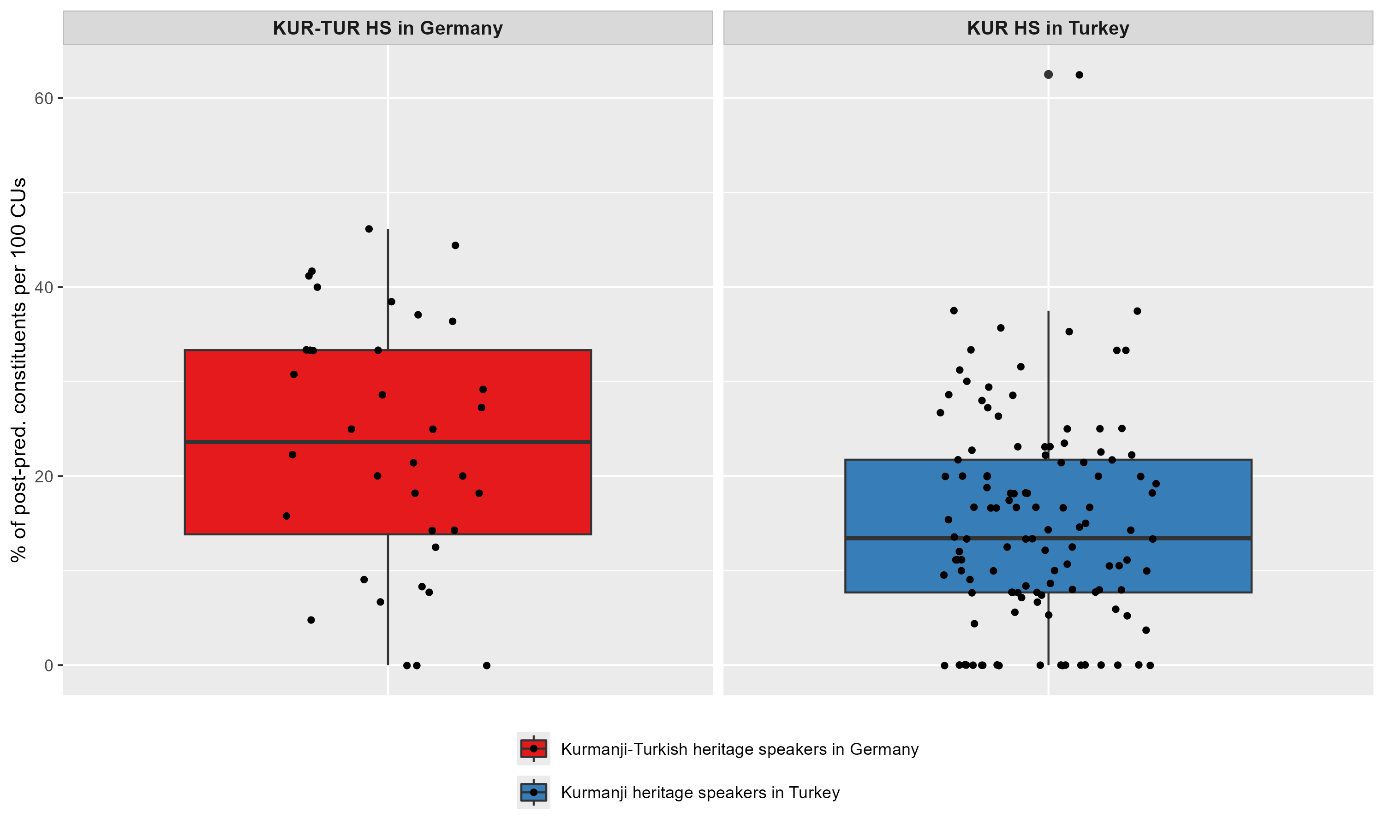
\includegraphics[width=\textwidth]{figures/iefremenko-img013.png}
\caption{\label{fig:key:14} Frequency distribution of post-predicate structures per 100 CUs.}
\end{figure}

\figref{fig:key:14} presents the frequency distribution of post-predicate structures in Kurmanji, normalized per 100 CUs, in Turkey and Germany. The line within each box shows the median, while each dot indicates the number of post-predicate structures used by a speaker in a communicative situation. Dots placed beyond the whiskers' range are outliers.

The figure reveals that the majority of utterances follow a verb-final word order. However, there is considerable individual variation among speakers: while some do not use the post-predicate position at all, others employ post-predicate structures in more than 60\% of their utterances. Additionally, the figure indicates that speakers in Germany use post-predicate structures more frequently than those in Turkey, with an average of 23.3 CUs per 100 containing a post-predicate constituent in Germany, compared to 14.9 CUs in Turkey.

To determine whether the difference in the use of post-predicate structures between the groups is significant, a linear mixed-effects model was conducted. The dependent variable is the Percentage of Post-Predicate Structures, the fixed effect is Group, while Participant is included as a random variable. The results of the regression are presented in \tabref{tab:key:10}.

\begin{table} \small
\begin{tabularx}{\textwidth}{XYY}
\lsptoprule
\textbf{Random effects:}\\
\midrule
% \lsptoprule
\textbf{Groups} & \textbf{Variance} & \textbf{Standard Deviation}\\
Participant (Intercept) & 29.5 & 5.43\\
Residual & 105.3 & 10.26\\
% \lspbottomrule
\midrule
\end{tabularx}
\begin{tabularx}{\textwidth}{Xrrrrr}
% \lsptoprule
\textbf{Fixed effects:}\\
\midrule
% \lsptoprule
\textbf{Fixed effect} & \textbf{Estimate} & \textbf{Std. Error} & \textbf{df}  & \textbf{t-value} & \textbf{\textit{p}-value}\\
Intercept & 23.27 & 2.49 & 37.00 & 9.34 & $<.0001^{***}$\\
Group (Tubi) & -8.39 & 2.83 & 37.00 & -2.95 & $.005^{**}$\\
\lspbottomrule
\end{tabularx}
\caption{Regression table for lmer with the dependent variable Percentage of Post-Predicate Structures and the independent variable Group.}
\label{tab:key:10}
\end{table}

Group: Group is an independent variable assigned the levels \textit{Kurmanji-Turkish HS in Germany (Detr)} and \textit{Kurmanji HS in Turkey (Tubi)}. As seen in \tabref{tab:key:10}, the result of the regression analysis shows that Kurmanji speakers in Turkey tend to employ significantly fewer post-predicate structures compared to Kurmanji speakers in Germany.

The analysis reveals that Kurmanji speakers in Germany use significantly more post-predicate constituents than those in Turkey. However, since the post-predicate position in Kurmanji is primarily reserved for certain indirect objects, it is not considered non-canonical. Moreover, the reasons behind the higher frequency of post-predicate constituents among speakers in Germany remain unclear. One possibility is that the distribution of these structures differs across communicative situations in each group, similar to patterns observed in Turkish. Another potential explanation could be differences in the types of post-predicate structures used by each group. To explore this further, the following sections present the analysis of the distribution of post-predicate structures across communicative situations and then focus on the different types of post-predicate constituents.

\section[The use of post-predicate constituents in Kurmanji]{The use of post-predicate constituents in Kurmanji across different communicative situations}\label{sec:key:6.2}

So far, the analysis indicates that heritage speakers of Kurmanji in Germany use more post-predicate structures than speakers in Turkey. To investigate whether communicative situations, i.e. formality and mode, affect the frequency differences between the groups, the frequency distribution of post-predicate structures was analyzed across four communicative contexts: informal spoken, informal written, formal spoken, and formal written. The results are presented in \figref{fig:key:15}.

\begin{figure}
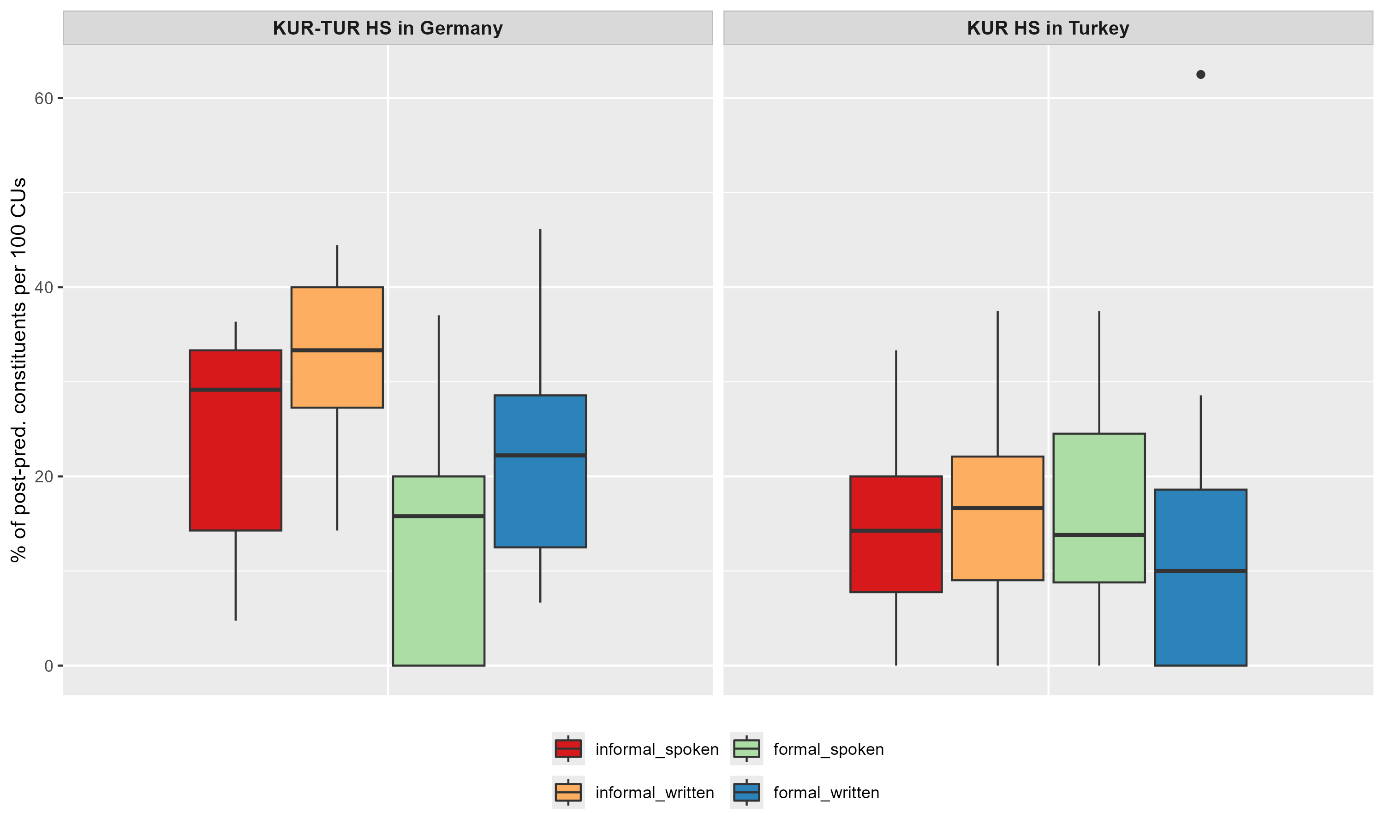
\includegraphics[width=\textwidth]{figures/iefremenko-img014.png}
\caption{\label{fig:key:15}Frequency distribution of post-predicate structures in Kurmanji in two country groups across different communicative situations.}
\end{figure}

\figref{fig:key:15} illustrates the frequency distribution of post-predicate structures across communicative situations in Turkey and Germany, normalized per 100 CUs. The line within each box shows the median, while the whiskers extended from the box indicate the minimum and maximum values. Dots falling outside the whisker range are outliers.

The visual patterns in the frequency distribution differ between the groups, and the descriptive means confirm these tendencies. For Kurmanji heritage speakers in Turkey, the use of post-predicate structures remains relatively consistent across communicative situations, with {means} ranging from $\bar{x}$ =12.62\% in the formal written situation to $\bar{x}$ =16.66\% in the formal spoken situations, and little difference between the informal spoken ($\bar{x}$={14.32\%}) and informal written ($\bar{x}$ = {15.91\%}) situations. In contrast, Kurmanji-Turkish heritage speakers in Germany show clearer situational differences. They employ post-predicate structures most frequently in the informal written context ($\bar{x}${=33.09}{\%}), followed by the informal spoken ($\bar{x}$ = {23.25\%}) and the formal written ($\bar{x}$ = {23.40\%}) situations, while the lowest mean is found in the formal spoken situations ($\bar{x}$ = {13.35\%}). Notably, speakers in Germany rely on the post-predicate position far more often in the informal written mode than in any other setting.

To determine the effects of formality and mode on the use of post-predicate structures among the two groups of Kurmanji speakers, a linear mixed-effects model was conducted. The dependent variable was the Percentage of Post-Predicate Structures, with fixed effects for the interaction between Formality (formal vs. informal) and Mode (spoken vs. written) nested within the variable Group. The variable Participant was included as a random effect. The results of the regression analysis are presented in \tabref{tab:key:11}.

\begin{table}[t]
\begin{tabularx}{\textwidth}{XYY}
\lsptoprule
\textbf{Random effects:}\\
\midrule
\textbf{Groups} & \textbf{Variance} & \textbf{Standard Deviation}\\
Participant (Intercept) & 32.68 & 5.71\\
Residual & 92.55 & 9.62\\
% \lspbottomrule
\midrule
\end{tabularx}
% \vspace{0.5em}
\begin{tabularx}{\textwidth}{lrrrrr}
% \lsptoprule
\textbf{Fixed effects:}\\
\midrule
% \lsptoprule
\textbf{Fixed effect} & \textbf{Estimate} & \textbf{Std. Error} & \textbf{df}  & \textbf{t-value} & \textbf{\textit{p}-value}\\
Intercept & 13.47 & 3.73 & 122.89 & 3.56 & $<.0001^{***}$\\
\addlinespace[0.5em]
Group (Tubi) & 3.31 & 4.25 & 122.89 & 0.78 & .43\\
\addlinespace[0.5em]
Group (Detr)\_\\Formality (informal) & 9.90 & 4.53 & 111.00 & 2.18 & $.03^{*}$\\
\addlinespace[0.5em]
Group (Tubi)\_\\Formality (informal) & -2.33 & 2.48 & 111.00 & -0.94 & .34\\
\addlinespace[0.5em]
Group (Detr)\_\\Mode (written) & 10.05 & 4.53 & 111.00 & 2.22 & $.03^{**}$\\
\addlinespace[0.5em]
Group (Tubi)\_\\Mode (written) & -4.04 & 2.48 & 111.00 & -1.63 & .10\\
\addlinespace[0.5em]
Group (Detr)\_\\Formality (informal)\_\\Mode (written) & -0.22 & 6.41 & 111.00 & -0.03 & .97\\
\addlinespace[0.5em]
Group (Tubi)\_\\Formality (informal)\_\\Mode (written) & 5.63 & 3.51 & 111.00 & 1.60 & .11\\
\lspbottomrule
\end{tabularx}
\caption{\label{tab:key:11}Regression table for lmer with the dependent variable Percentage of Post-Predicate Structures and the independent variables Formality and Mode.}
\end{table}

Formality: Formality is a binary independent variable categorized as \textit{formal} and \textit{informal} in this study. As shown in \tabref{tab:key:11}, formality significantly influences the use of post-predicate structures in Kurmanji speakers in Germany, with the speakers tending to employ post-predicate constituents more frequently in the informal communicative situations.

Mode: Mode is also a binary independent variable, consisting of \textit{spoken} and \textit{written} categories. Similar to formality, mode affects the use of the post-predicate position, but this influence is observed only among Kurmanji speakers in Germany, where the speakers are more likely to use the post-predicate position in the written communicative situations.

Thus, the regression analysis confirms the observations from the plot: while in Kurmanji speakers in Turkey mode and formality do not have an effect on the employment of the post-predicate position, Kurmanji speakers in Germany are more likely to use the post-predicate position in the informal and written communicative situations. The findings from the Kurmanji group in Turkey are not surprising, as the use of the post-predicate position in Kurmanji is determined by predicate semantics and is therefore not expected to be subject to register variation. In contrast, the observations in Kurmanji speakers in Germany are interesting and challenging to explain. While the increased use of post-predicate constituents in the informal communicative situations aligns with the patterns found in Turkish and reported in studies on German, the higher frequency of these structures in the written situations compared to the spoken ones remains unclear. However, it is important to note that the number of speakers in this group is smaller than in the other groups, suggesting that the observed frequencies could change with more data.

\section{Types of post-predicate constituents in Kurmanji}\label{sec:key:6.3}

The analysis now moves to the types of post-predicate constituents in Kurmanji. As stated in \sectref{sec:key:3.3}, the use of the post-predicate position in Kurmanji is reserved for certain indirect objects, namely, locational goals of verbs of motion and verbs of caused motion, goals of verbs of transfer and addressees of verbs of speech (\citealt{Haig2014, HaigThiele2014, Haig2018, Gundogdu2019}). The following section examines the extent to which argument type influences the use of the post-predicate position in Kurmanji. Additionally, the analysis explores whether the more frequent use of post-predicate structures among speakers in Germany, compared to those in Turkey, is driven by differing preferences for argument types in the post-predicate position.

\begin{figure}
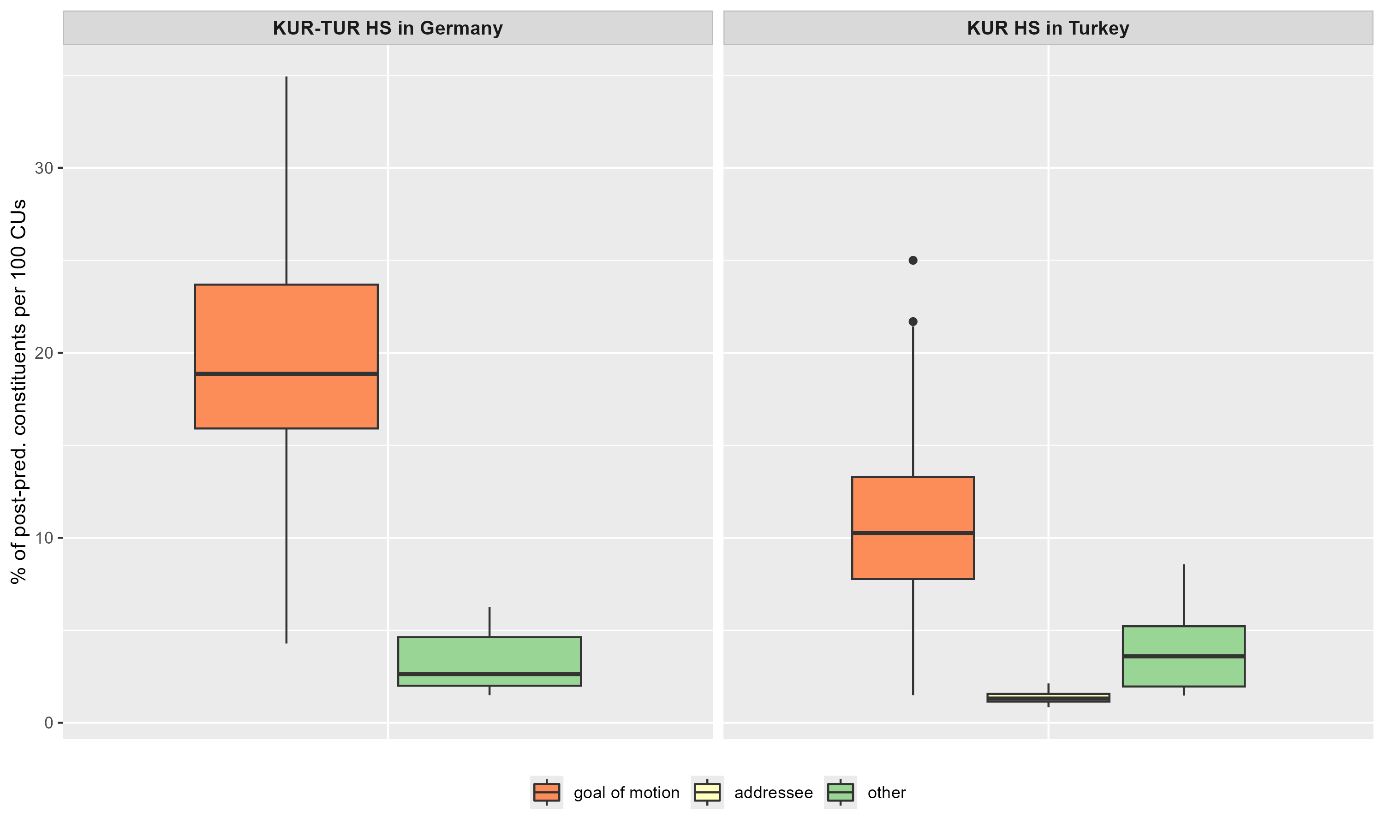
\includegraphics[width=\textwidth]{figures/iefremenko-img015.png}
\caption{\label{fig:key:16}Types of post-predicate structures in Kurmanji in two country groups.}
\end{figure}

\figref{fig:key:16} presents the frequency distribution of different types of arguments in the post-predicate position in Kurmanji as spoken in Turkey and Germany, normalized per 100 CUs. The line inside each box represents the median, while the whiskers extend to the minimum and maximum values. Dots falling outside the whisker range indicate outliers.

The figure visualizes two of the three possible types of arguments: goals of motion (shown in orange) and addressees of verbs of speech (shown in yellow). The third type—recipients of verbs of transfer—occurs very rarely in the dataset, as the video shown to participants did not elicit the use of transfer verbs. Consequently, as seen in \figref{fig:key:16}, no instances of recipients of verbs of transfer appear in the post-predicate position.

Beyond these argument types, the analysis shows that other constituents can also appear post-predicatively in Kurmanji (shown in green). These will be discussed later in this chapter (\sectref{sec:key:6.3.6}).

The descriptive means confirm that in both country groups, goals of motion are the most frequent type in the post-predicate position. For Kurmanji heritage speakers in Turkey, goals of motion appear with $\bar{x}${=11.33}{\%}, followed by other constituents ($\bar{x}$={4.01\%}) and addressees of speech ($\bar{x}$={1.40\%}). In contrast, Kurmanji-Turkish heritage speakers in Germany use goals of motion more frequently overall ($\bar{x}$={19.61\%}), while other constituents occur with $\bar{x}$={3.30\%}, no addressees of verbs of speech are attested in this group. However, these differences in frequency distribution across argument types do not necessarily reflect the general distribution of post-predicate constituents in Kurmanji. Rather, they may partly result from the data collection method: the video shown to participants featured significant movement, minimal interaction, and virtually no transfer between the actors. As a result, the data predominantly show goals of motion, followed by addressees of speech, with almost no occurrences of recipients.


\subsection{Goals of motion and caused motion}\label{sec:key:6.3.1}

The following section takes a closer look at the goals of motion and caused motion found in the data. As outlined in \sectref{sec:key:3.3}, goals of motion in Kurmanji can be flagged either with the oblique case or an adposition. Notably, these two types differ in their placement relative to the verb. Case-flagged goals must appear immediately after the predicate and cannot precede it (\citealt{Haig2014, Gundogdu2019}). In contrast, the position of adpositional goals is more flexible and depends on the type of adposition and the dialect \citep{Haig2014}. \citet{Asadpour2021} further highlights that beyond flagging and regional variation, additional factors influence the positioning of goal arguments, with information structure playing a particularly significant role. However, these findings are based on Mukri Kurdish, spoken in Iran. Hence, this section will explore the effects of factors such as flagging, formality and mode and information structure on the employment of goals of (caused) motion in the post-predicate position.

First, the analysis focuses on flagging, presenting the frequency distribution of the most common argument type in the data: goals of verbs of motion and caused motion. These goals are marked either by case or an adpositional phrase and can appear before or after the predicate.

\begin{figure}
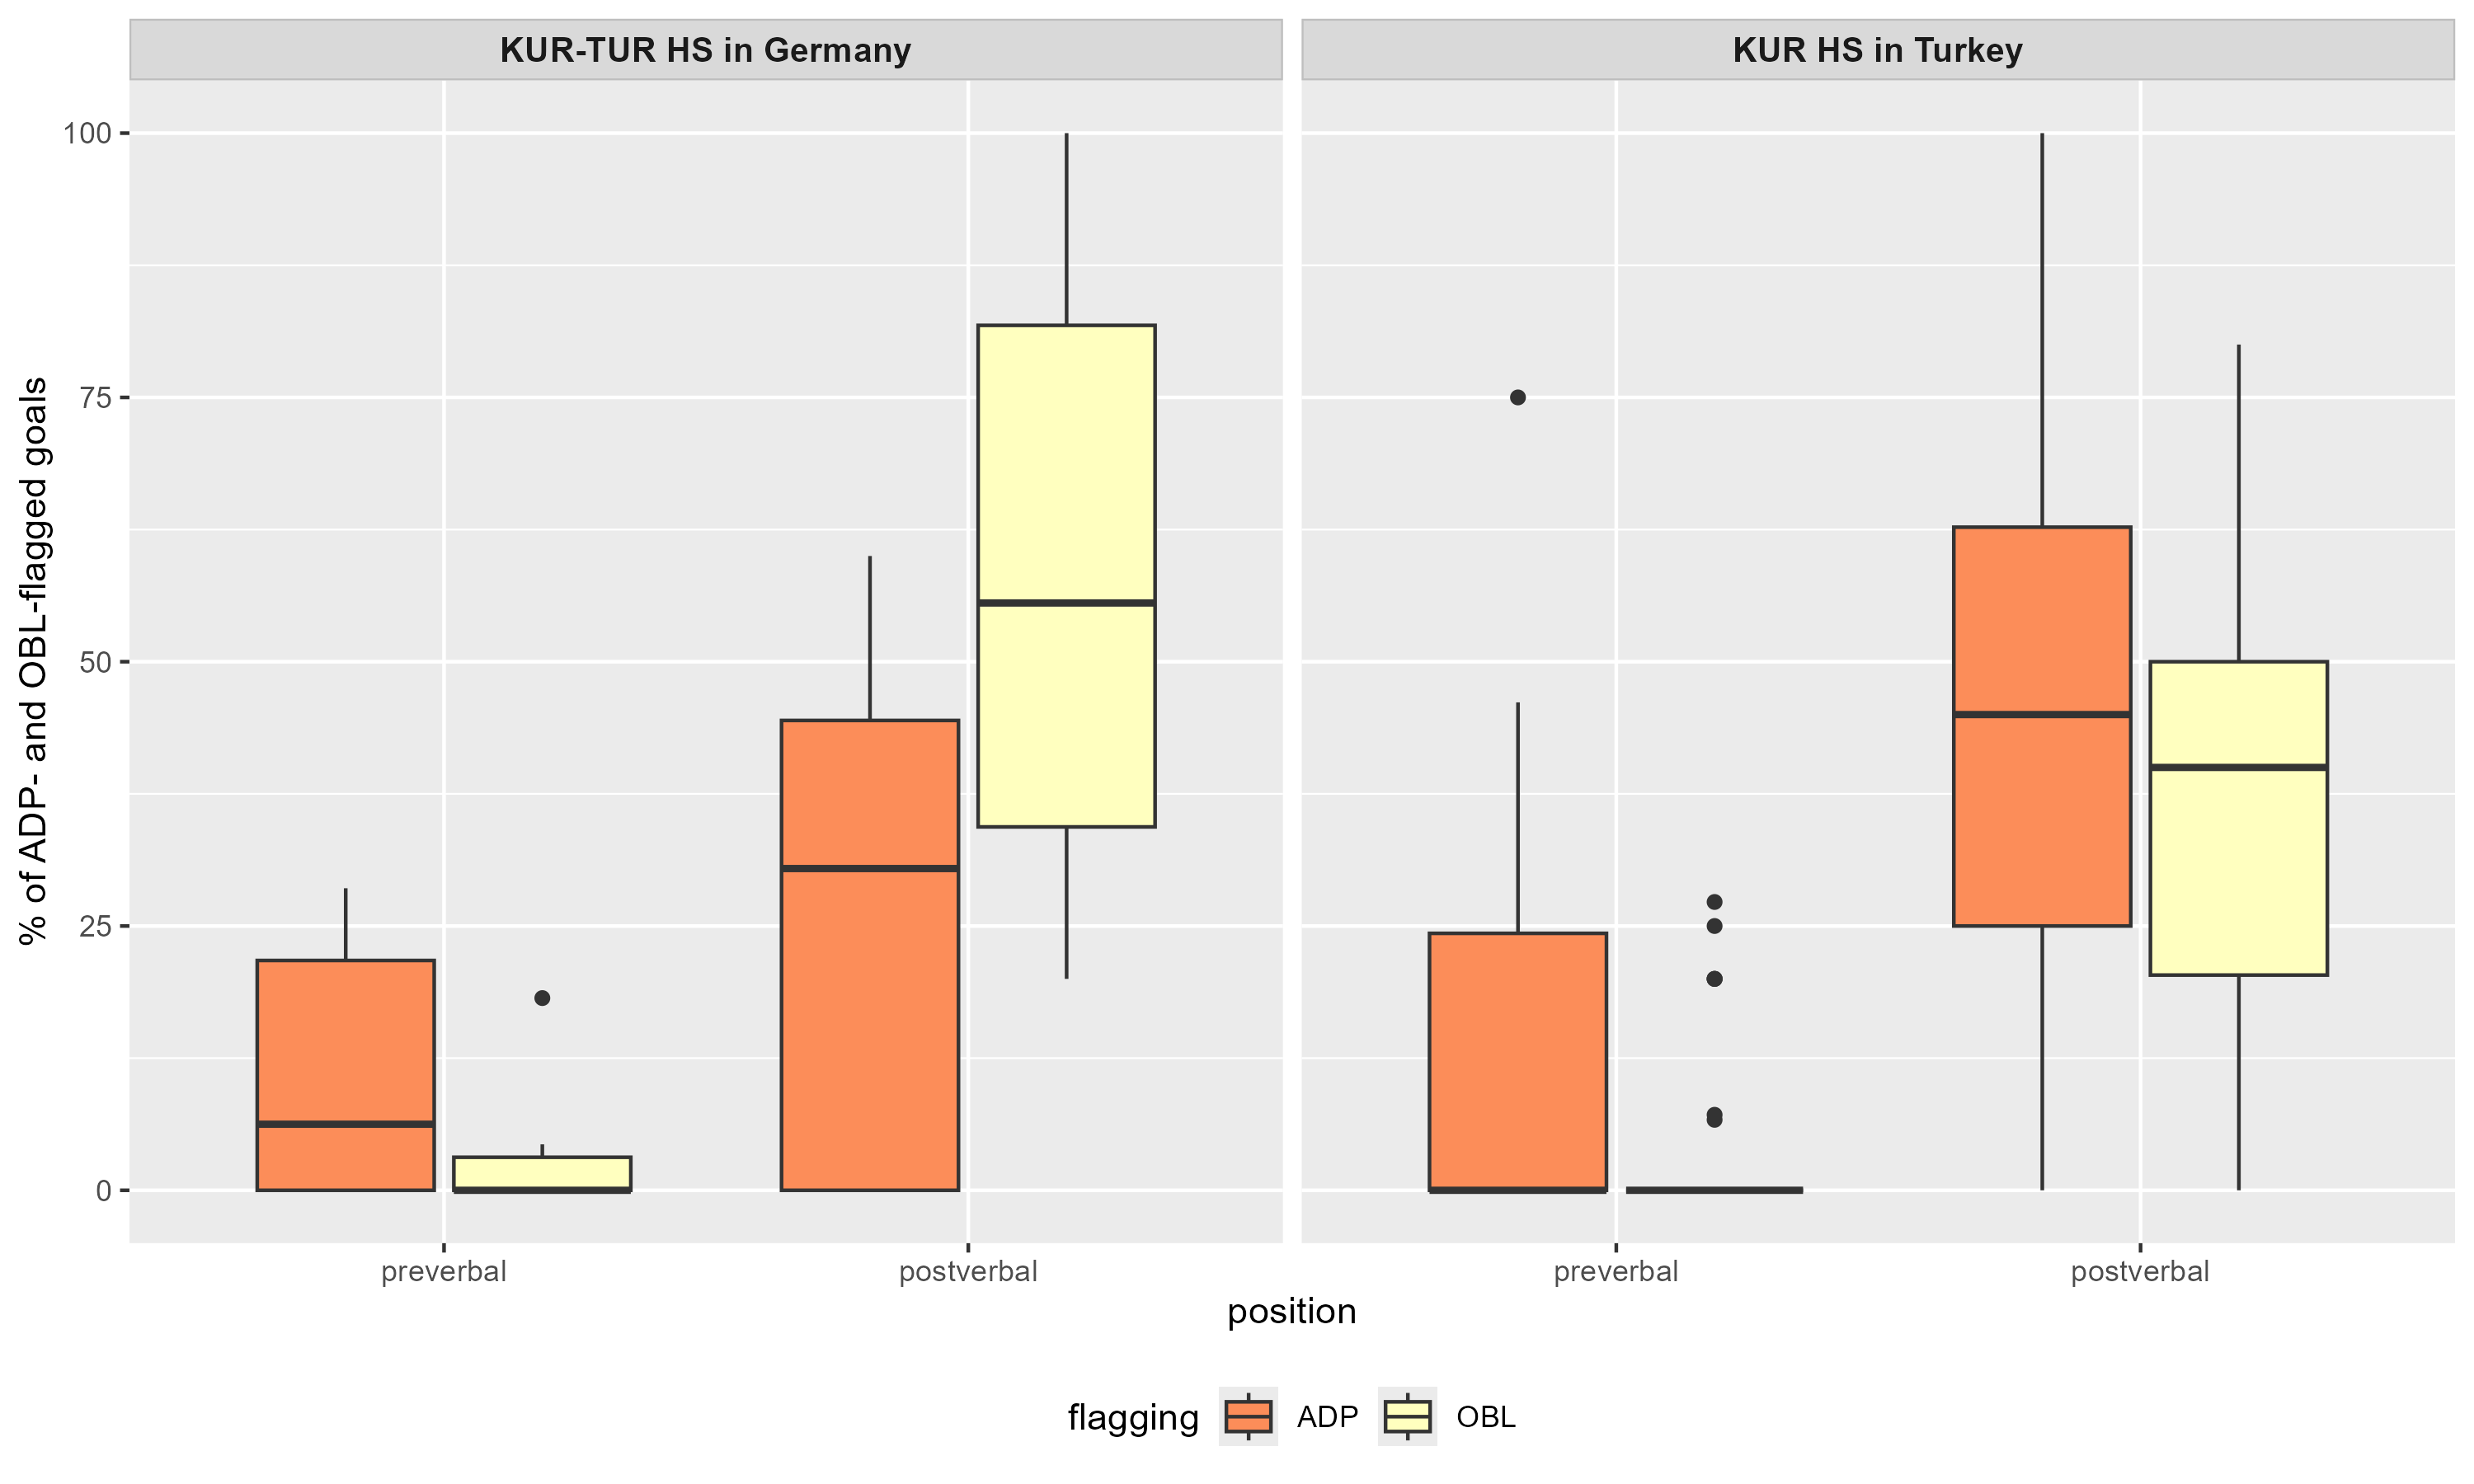
\includegraphics[width=\textwidth]{figures/iefremenko-img016.png}
\caption{\label{fig:key:17}Frequency distribution of goals of motion flagged with oblique case (OBL) or an adposition (ADP) in two country groups.}
\end{figure}

\newpage
\figref{fig:key:17} illustrates the frequency distribution of goals of motion, flagged with either the oblique case (OBL) or an adposition (ADP), and positioned in the pre- or post-predicate. The frequency of each type of flagging is calculated in relation to the total number of goals of motion within the data from each country group.

The figure shows that Kurmanji speakers in both countries use both types of flagging. Regarding the position of goals of motion, the post-predicate position is favored for both types of flagging among both speaker groups. In Germany, ADP-marked goals occur postverbally with $\bar{x}${=27.59\%} and preverbally with $\bar{x}$={11.28\%}, while OBL-marked goals occur postverbally with $\bar{x}$={58.28\%} and preverbally with $\bar{x}$={2.85\%}. In Turkey, ADP-marked goals appear postverbally with $\bar{x}$={46.66\%} and preverbally with $\bar{x}$={13.32\%}, and OBL-marked goals occur postverbally with $\bar{x}$={35.82\%} and preverbally with $\bar{x}$={4.20\%}. Taken together, these means indicate that in Germany, case flagging (OBL) is preferred overall, with $\bar{x}$={58.28\%} of goals flagged with case compared to $\bar{x}$={27.59\%} flagged with an adposition (ADP). Conversely, in Turkey, speakers favor adpositional flagging, with $\bar{x}$={46.66\%} of goals flagged with an adposition versus $\bar{x}$={35.82\%} flagged with case.


Since flagging is the factor influencing the placement of goals in Kurmanji, the following discussion will address the two types of flagging separately.

\subsubsection{Goals of motion flagged with case}\label{sec:key:6.3.1.1}

As stated in \sectref{sec:key:3.3}, case-flagged goals in Kurmanji are licensed in the post-predicate position (\citealt{Haig2014, Haig2018, Gundogdu2019}), and the data clearly show that they are predominantly used post-predicatively. For instance, in \REF{ex:key:55}, the goal argument \textit{tope} ‘to the ball’ is placed after the verb \textit{avêtin} ‘to throw’.

\ea%55
  \label{ex:key:55} Kurmanji, TUbi29MK\_isK \\
\gll Kûçik   xe     avêt-e       top-e \\
dog  oneself    throw.\textsc{pst.3sg}-\textsc{drct}  ball-\textsc{obl.f}\\
\glt ‘The dog threw itself to the ball’ 
  \z

However, the data indicate that Kurmanji speakers in both Turkey and Germany also place case-flagged goals in the pre-predicate position, as illustrated in examples \REF{ex:key:56} and \REF{ex:key:57}.

\ea%56
  \label{ex:key:56} Kurmanji,  TUbi18MK\_isK \\
\gll Ji   dest-ê     xwê   iii   sêv   erd-ê     ket\\
from  hand\textsc{-ez.m}   own  hm  apple   ground\textsc{-obl.m} fell.\textsc{pst.3sg}\\
\glt ‘Apple fell down from her hands on the ground’
  \z

\ea%57
  \label{ex:key:57} Kurmanji, TUbi10MK\_fsK \\
\gll {Gog   ewk   bû     iii ling-ê     merik-ê   ket}\\
ball  thing   be.\textsc{pst.3sg}  hm  {} foot-\textsc{ez.m}  man-\textsc{obl.m}  fell.\textsc{pst.3sg}\\
\glt ‘Ball well was hmm, fell to the man’s foot’  
  \z

In examples \REF{ex:key:56} and \REF{ex:key:57}, the goal arguments \textit{erdê} `on the ground' and \textit{lingê merikê} `on the man's foot' are positioned immediately before the predicate. Previous research on word order in Kurmanji (\citealt{Haig2014, Haig2018, Gundogdu2019}) classifies such constructions as non-canonical because goal arguments can only occupy the pre-predicate position if they are adpositionally flagged. For instance, including the preposition \textit{li} `in' before the goal arguments in examples \REF{ex:key:56} and \REF{ex:key:57} would render the sentences canonical, as demonstrated in examples \REF{ex:key:58} and \REF{ex:key:59}.

\ea
    \label{ex:key:58} Kurmanji, self-constructed \\
\gll * Ji   dest-ê     xwê   iii   sêv   li  erd-e     ket\\
{} from  hand-\textsc{ez.m}   own  hm   apple   in  ground\textsc{-obl.m} fell.\textsc{pst.3sg}\\
\glt \, ‘Apple fell down from her hands to the ground.’ 
    \z

\ea
    \label{ex:key:59} Kurmanji, self-constructed \\
\gll * Gog   ewk   bû     iii li  ling-ê     merik-ê      ket\\
{} ball  thing   be.\textsc{pst.3sg}  hm  {} in  foot-\textsc{ez.m}  man-\textsc{obl.m}  fell.\textsc{pst.3sg} \\
\glt \, ‘Ball well was hmm, fell to the man’s foot.’
    \z

If an argument is case-flagged, it should be positioned in the post-predicate location, as Kurmanji allows at most two case-flagged noun phrases (the subject and direct object) in the pre-predicate position (\citealt{Gundogdu2019}). Placing case-flagged goals immediately before the predicate may alter their intended meaning. Therefore, from a grammatical perspective, the case-flagged goals in examples  \REF{ex:key:58} and \REF{ex:key:59} can be interpreted as direct objects due to their placement in the pre-predicate position.

Although the absolute number of sentences featuring case-flagged goals in the pre-predicate position is relatively low, the data reveal that this placement is present in the speech of both groups. Specifically, there are 12 instances from the data of Kurmanji-Turkish bilinguals in Turkey, accounting for 4.20\% of all goals of motion in that group. In contrast, the data from Kurmanji-Turkish heritage speakers in Germany include four instances, representing 2.85\% of all goals of motion in that group.

A closer analysis of the examples from Kurmanji-Turkish bilinguals in Turkey reveals a consistent pattern in the use of verbs with case-flagged goal arguments in the pre-predicate position. Specifically, 11 out of the 12 instances of case-flagged goals in this preverbal position were used with the verb \textit{ketin} ‘to fall,’ as shown in example \REF{ex:key:56} and \REF{ex:key:57}, while one instance was used with the verb \textit{firîn} ‘to fly.’

Furthermore, the examples with the verb \textit{ketin} ‘to fall’ can be categorized into two groups: those featuring body parts as arguments (\textit{dest} ‘hand’ or \textit{ling} ‘foot’) and those where the argument is the goal \textit{erd} ‘ground.’ The first group includes six instances, where the examples suggest that the ball falls into the man's hands or feet. However, the video shows that the ball falls from the man's hands onto the road. This implies that the preposition \textit{ji} ‘from’ may be omitted or reduced, indicating that the constituents in the pre-predicate position are not actually goals but rather sources of motion, as shown in example \REF{ex:key:60}. Similarly, the example with the verb \textit{firîn} ‘to fly’ also includes the argument \textit{dest} ‘hand’ in the pre-predicate position. These instances, which can be interpreted as sources of motion, further explain their noncanonical placement before the verb, as sources of motion in Kurmanji are typically positioned in the preverbal position.

\ea
  \label{ex:key:60} Kurmanji, Tubi09MK\_iwK \\
     \gll Nişkava   gog   dest-ê     wî   ket \\
suddenly  ball  hand-\textsc{ez.m}  her  fall.\textsc{pst.3sg}\\
\glt ‘Suddenly the ball fell from his hands’ 
  \z

Example \REF{ex:key:60} is a written instance from a Kurmanji speaker in Turkey, where the argument \textit{destê wî} ‘her hand’ actually implies a source of action, suggesting that the preposition \textit{ji} ‘from’ has been omitted. Omitting a preposition is a phenomenon sometimes observed in the data of Kurmanji-Turkish bilinguals in Turkey. For instance, in \REF{ex:key:61}, the verb \textit{vegerandin} ‘to return’ implies motion away from a source. Therefore, the locative noun phrase is expected to be marked as a source of motion, not as a goal, as in the example.

\ea
  \label{ex:key:61} Kurmanji, TUbi04MK\_fwK \\
\gll Dema    ez     zanîngeh-ê          ve-di-geriya-m\\
while    I      university\textsc{-obl.f}     \textsc{prfx-prs-}return-\textsc{1sg}\\
\glt ‘While I was coming back (from) the college…’ 
  \z

The tendency to omit prepositions may arise from convergence effects with the majority language, Turkish, which does not use prepositions in the same way. This phenomenon is similarly observed in Turkish child heritage speakers in Germany \citep{Turgay2010} and in L1 Turkish learners of English and German (\citealt{Ozisik2014, Yildiz2016}). These studies indicate that L1 Turkish speakers often omit prepositions when using their L2, whether it be German or English, both of which are prepositional languages. In contrast to these findings, example \REF{ex:key:61} suggests a possible influence of L2 Turkish on the use of L1 Kurmanji.

Considering the six examples with the verb \textit{ketin} ‘to fall’ that feature a body part as instances of the source of motion, there are five remaining examples with the case-flagged goal \textit{erdê} ‘onto the ground’ placed before the verb \textit{ketin} ‘to fall.’ It is important to note that this construction is only found in the data from Kurmanji-Turkish bilinguals in Turkey. In Turkish, \textit{erdê ketin} is expressed as \textit{yere düşmek}, which translates literally to ‘to fall on the ground.’ This expression is a fixed construction in Turkish, where \textit{yer-e} (ground-\textsc{dat}) in \textit{yere düşmek} (ground-\textsc{dat} fall.\textsc{inf}) cannot be placed in the post-predicate position and is always directly attached to the verb. This observation is corroborated by the RUEG data, a search for the construction \textit{yere düşmek} revealed that all instances occur in the immediate pre-predicate position. This result is based on ten occurrences of the construction in the Turkish of Kurmanji-Turkish bilingual speakers, eight instances of \textit{yere düşmek} in Kurmanji-Turkish heritage speakers in Germany \citep{IefremenkoEtAl2024}, and 19 occurrences in the Turkish of monolingual speakers \citep{LudelingEtAl2024}. Thus, the noncanonical position of the argument \textit{erdê} in Kurmanji may be attributed to the direct copying of the entire construction from Turkish. This finding will be further discussed in \sectref{sec:key:7.1}.

However, beyond the cross-linguistic explanation, the noncanonical position may also be influenced by the verb \textit{ketin} itself. In Kurmanji, there are constructions where \textit{ketin} functions as a light verb, lacking its full meaning, as seen in phrases like \textit{bi rê ketin} ‘to set off (on a journey)’ and \textit{li ber ketin} ‘to meet/to encounter.’ This could account for the higher frequency of construction copying observed with the verb \textit{ketin}, although it does not fully explain the noncanonical position of the case-flagged goal \textit{erdê}.

Additionally, it is essential to note that the noncanonical construction with a goal argument in the pre-predicate position does not dominate in Kurmanji usage. Most speakers still place case-flagged goals, including \textit{erdê}, in the post-predicate position. In the Kurmanji data from heritage speakers in Turkey, the construction ‘to fall on the ground’ has been used 20 times, with 15 instances being canonical (featuring a postposed argument) and five instances being noncanonical (with the argument in the pre-predicate position). Furthermore, even speakers who occasionally place the argument \textit{erdê} in the pre-predicate position in one communicative situation employ the canonical post-predicate position in other communicative situaitions. For instance, one female speaker placed the goal \textit{erdê} in the immediate pre-predicate position during the informal spoken production (see example \REF{ex:key:62}) but used it in the canonical post-predicate position in the written mode (see example \REF{ex:key:63}).

\ea \label{ex:key:62} Kurmanji, TUbi19FK\_isK \\
\gll Pişte    zilam   iii   gok-ê    xwe imm (--)   ji   dest-ê     xwa\\
afterwards  man  hm  ball-\textsc{ez.f}  \textsc{refl}  hmm  {} from  hand\textsc{-ez.m}  \textsc{refl} \\
\gll imm (--)   erd-ê       ket \\
hmm   {} ground-\textsc{obl.m}    fall.\textsc{pst.3sg}\\
\glt ‘Afterwards the man hmm his ball hmm (--) fell from his hand hmm (--) to the ground.’ 
\z


\ea
  \label{ex:key:63} Kurmanji, TUbi19FK\_iwK \\
\gll Gok-ê     zîlam   ji   dest-e    wî   ket     ard-ê \\
ball-\textsc{obl.f}  man  from  hand\textsc{-ez.m}  his  fall.\textsc{pst.3sg}  ground-\textsc{obl.m}\\
\glt ‘The man's ball fell from his hand onto the ground.’ 
  \z

Regarding the Kurmanji speakers in Germany, the relatively low absolute number of noncanonically placed arguments may be attributed to the fact that the data come from only nine speakers, resulting in fewer instances compared to Kurmanji-Turkish speakers in Turkey. Specifically, there are four case-flagged goals positioned pre-predicatively, produced by three speakers. Interestingly, unlike the Kurmanji speakers in Turkey, there is greater variation in the verbs that accommodate case-flagged arguments in the preverbal position among the speakers in Germany. These speakers employ pre-predicate goals with a range of verbs, including \textit{xistin} ‘to hit,’ \textit{lêxistin} ‘to beat/to hit,’ \textit{bazdan} ‘to run,’ and \textit{kirin} ‘to do.’

Examining these examples more closely reveals that two instances originate from the same speaker and exhibit code-switching from Turkish to Kurmanji. In these sentences, the goal is expressed in Turkish, while the verb is in Kurmanji (see examples \REF{ex:key:64} and \REF{ex:key:65}). Notably, the goal argument is a cognate of the Turkish word for ‘car’ (\textit{araba}), leading to ambiguity regarding whether the argument is in Kurmanji or Turkish. However, given that the data is written, the participant’s spelling suggests that the argument is the Turkish noun \textit{araba}. Consequently, the pre-predicative placement of the goal argument in examples \REF{ex:key:64} and \REF{ex:key:65} may be influenced by the Turkish structure of the utterance, with only the verb being in Kurmanji. From the perspective of canonical Turkish, placing a goal constituent in the pre-predicate position is a normative practice.

\ea \label{ex:key:64} Kurmanji, TUbi06MK\_fwK \\
\gll Alışveriş-e   araba-ya   di-kin  \\
grocery-\textsc{obl}  car-\textsc{dat}  \textsc{prs}-do\textsc{.3sg}\\
\glt ‘She was putting groceries into the car.’ 
\z

\ea
  \label{ex:key:65} Kurmanji and Turkish, TUbi06MK\_fwK \\
     \gll Arka-daki   araba   da   ön-deki   araba-ya   lexe \\
back\textsc{-attr}  car  also  front-\textsc{attr}  car-\textsc{dat}  bump\textsc{.pst.3sg}\\
\glt ‘The car at the back hit the car at the front.’ 
  \z

Thus, only two examples remain: in one instance, the verb \textit{bazdan} ‘to run’ takes a pre-predicative goal argument (see example \REF{ex:key:66}), while in the other, the verb \textit{xistin} ‘to hit’ features a goal argument in the pre-predicate position (see example \REF{ex:key:67}).

\ea
  \label{ex:key:66} Kurmanji, TUbi01FK\_isK \\
     \gll Zilam   pêşi-yê   bazda\\
man  front-\textsc{obl}  run\textsc{.pst.3sg}    \\
\glt ‘The man ran ahead.’ 
  \z

\ea
  \label{ex:key:67} Kurmanji, TUbi03FK\_isK \\
\gll Jî  ereba  pêşi-yê    xist\\
also  car  front-\textsc{obl}  hit.\textsc{pst.3sg}\\
\glt ‘He also hit the front car.’ 
  \z

Thus, the analysis revealed that in Kurmanji heritage speakers in Germany, there are only two instances of case-flagged goals placed in the noncanonical pre-predicate position. Furthermore, unlike in the cases observed among Kurmanji-Turkish bilinguals in Turkey, there is no specific verb or construction that prompts this noncanonical argument placement. This finding will be further explored in \sectref{sec:key:7.1}.

\subsubsection{Adpositional goals of motion}

As discussed in \sectref{sec:key:6.3.1}, both groups in the data show a preference for using adpositional goals in the post-predicate position rather than in the pre-predicate position. Previous studies by \citet{Haig2014} and \citet{Gundogdu2019} also indicate that adpositional goals predominantly appear post-predicate, though their placement can vary depending on the type of adposition and the dialect.

The following section presents the results of the frequency analysis for goals of motion flagged by different types of adpositions, calculated in relation to the total number of adpositional goals of motion within each speaker group (see \figref{fig:key:18}). For this analysis, five types of adpositionally flagged goals are categorized: those flagged by a basic preposition, those flagged with a locational noun, those that combine a basic preposition with a locational noun, those flagged by a postposition, and those flagged by a circumposition.

\begin{figure}
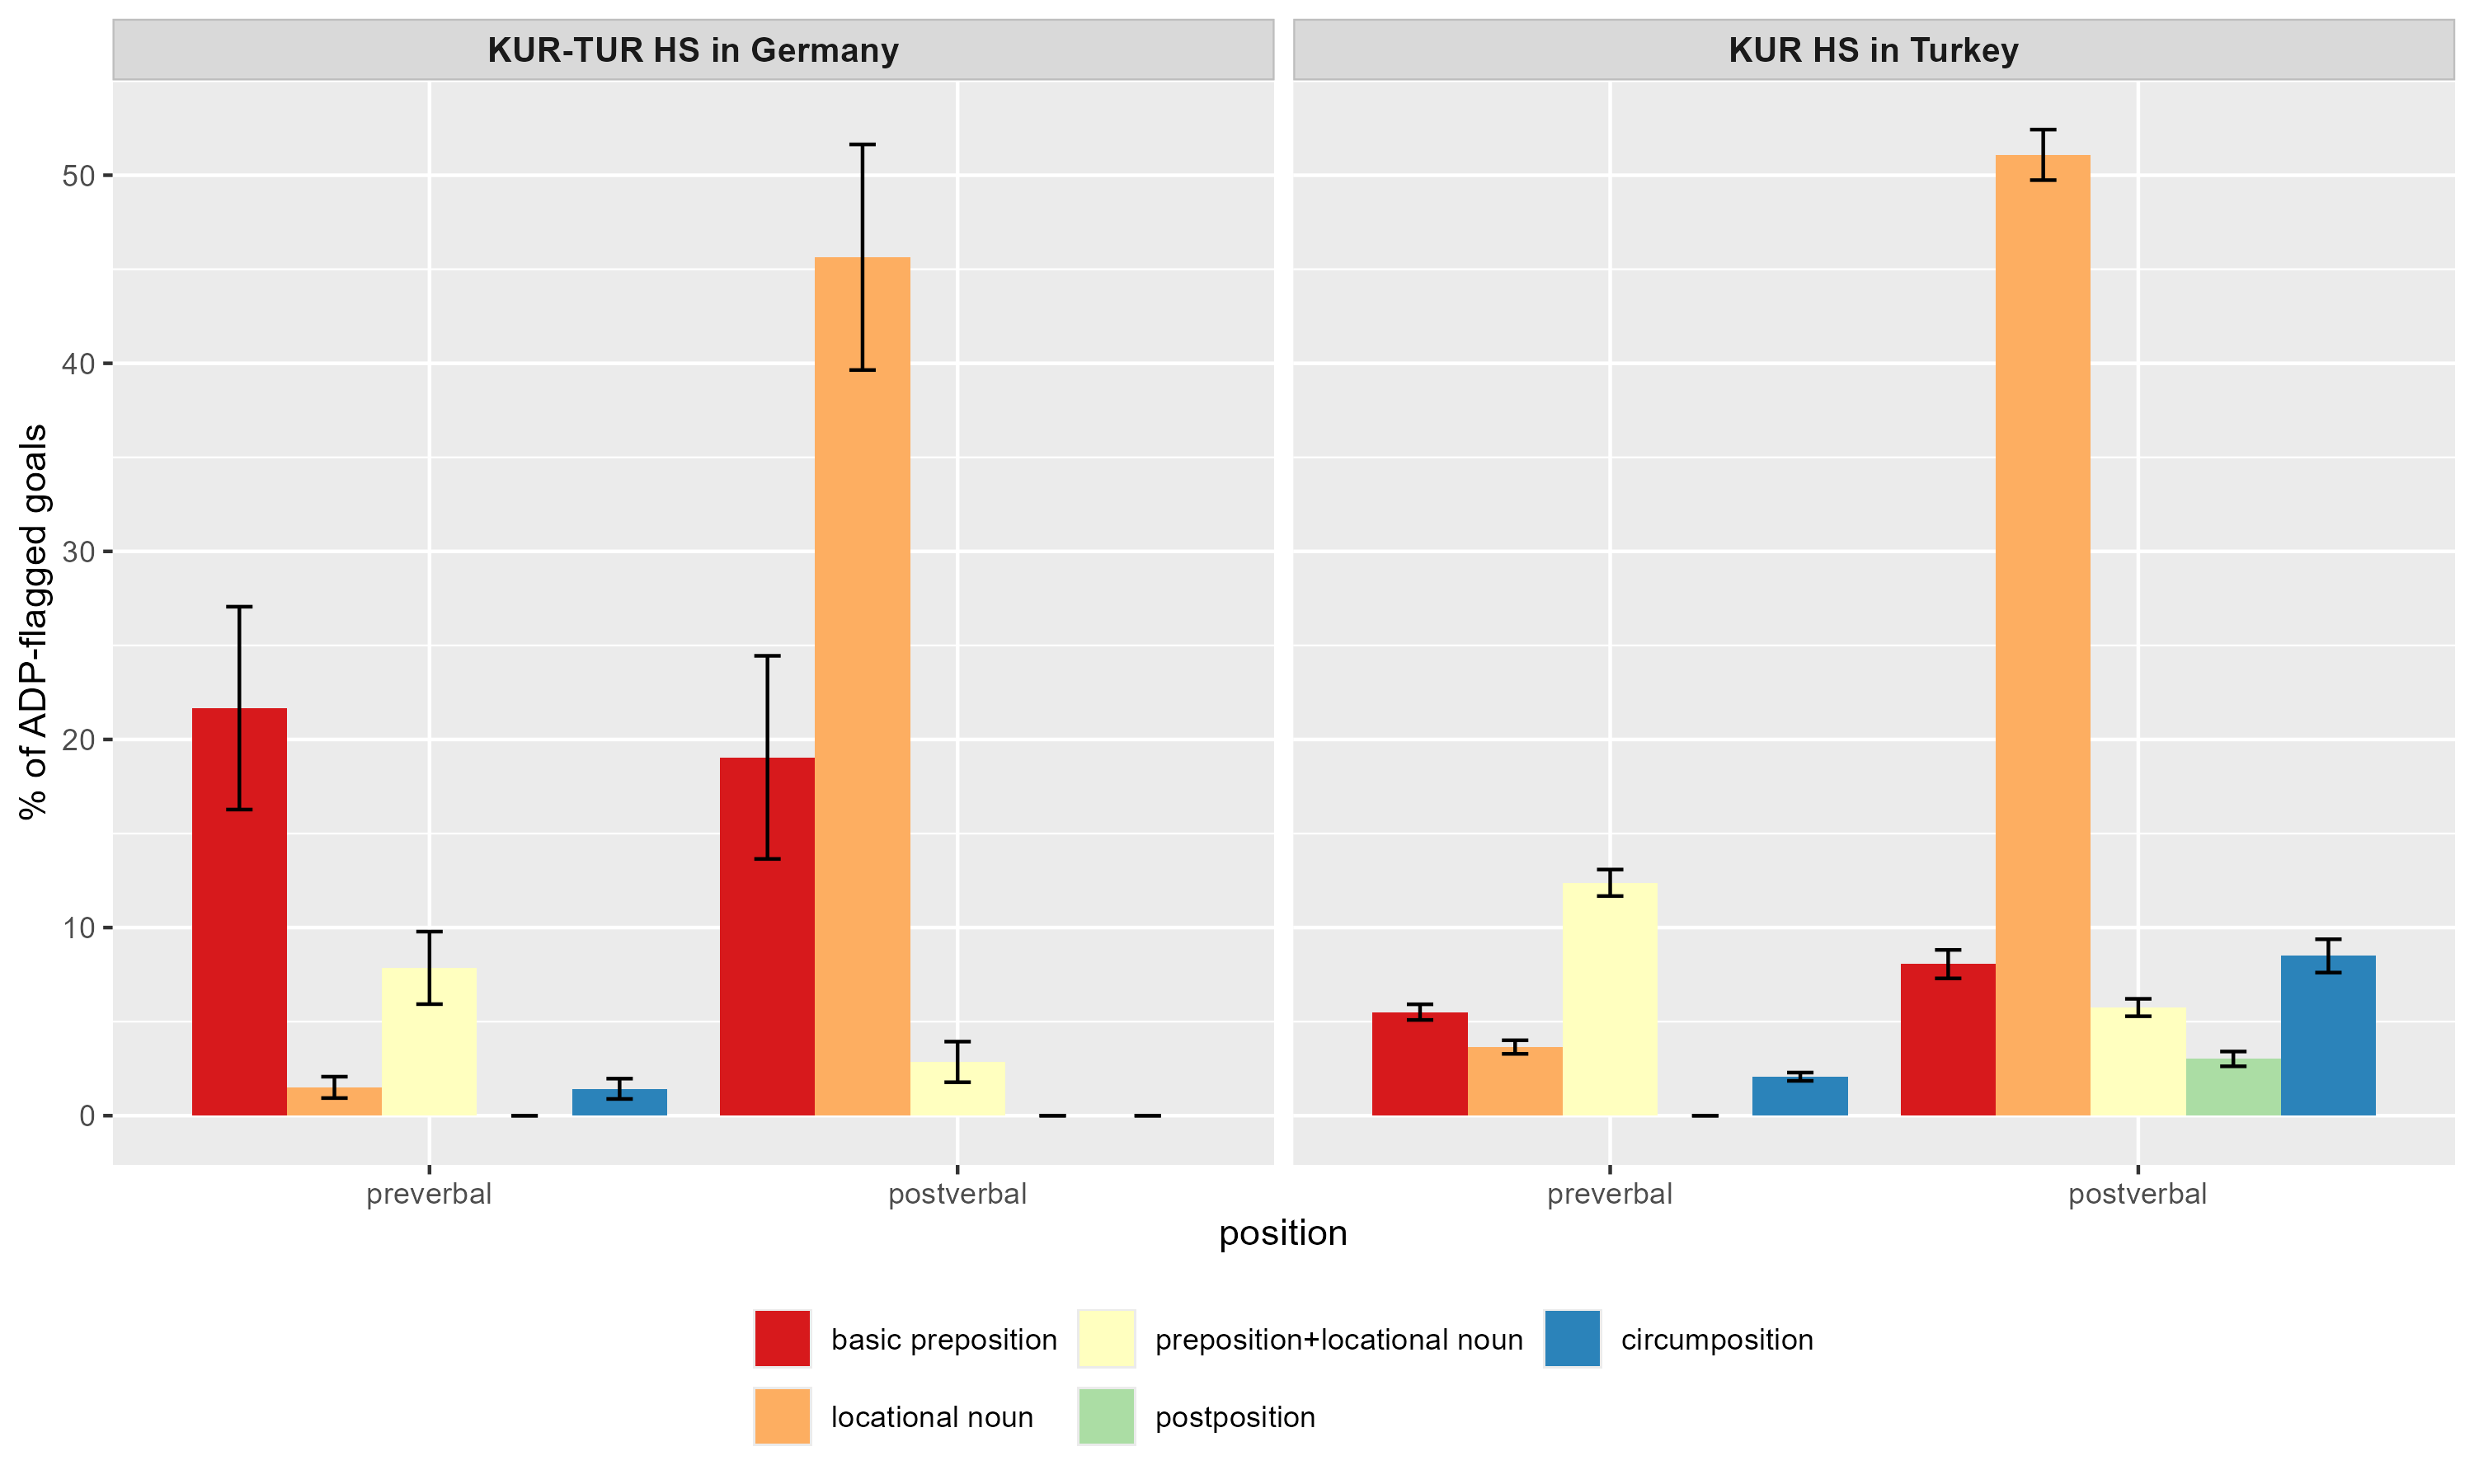
\includegraphics[width=\textwidth]{figures/iefremenko-img017.png}
\caption{\label{fig:key:18}Frequency of goals of motion flagged with different types of adpositions.}

\end{figure}

\figref{fig:key:18} illustrates the frequency distribution of goals of motion flagged by different types of adpositions, relative to the total number of adpositional goals of motion within each speaker group. Error bars represent standard error to enhance the precision of the mean estimates, particularly since some adposition types have low absolute counts.

Notably, \figref{fig:key:18} indicates that Kurmanji speakers predominantly use locational nouns as adpositions to express goals of motion. When combining occurrences in both post- and pre-predicate positions, 54.73\% of adpositional goals in Turkey and 47.14\% in Germany are flagged by locational nouns. As highlighted in \sectref{sec:key:3.3.1}, goals flagged with locational nouns are consistently placed in the post-predicate position because they are grammaticalized nouns. While the data primarily show that these goals are placed post-predicatively, there are some instances in both groups where such goals appear in the pre-predicate position.

\tabref{tab:key:12turkey} and \tabref{tab:key:12germany} present the absolute numbers of the different types of adpositions used in either the pre- or post-predicate position within the data.

% {\small
% \begin{longtable}
% {l p{2cm} l@{}r r }
% \caption{\label{tab:key:12turkey}The absolute number of different types of adpositions in the pre- and post-predicate position in the Turkey data.}\\
% \lsptoprule
% Group & Adposition type & Name & Pre-predicate & Post-predicate\\
% \midrule
% \endfirsthead
%
% \lsptoprule
%  Group & Adposition type & Name & Pre-predicate & Post-predicate\\
% \midrule
% \endhead
%
% \lspbottomrule
% \endlastfoot
%
% \tablevspace
% Kurmanji & \multirow{3}{2cm}{Basic prepositions} & \textit{bo} ‘to’ & 0 & 2\\
% HS in &  & \textit{li} ‘in’ & 12 & 3\\
% Turkey &  & \textit{pê} ‘to/into’ & 0 & 1\\
% \tablevspace
% \cline{2-5}
% \tablevspace
% \quad & \multirow{8}{2cm}{Locational nouns} & \textit{ber} ‘front’ & 1 & 14\\
% \quad &  & \textit{bin} ‘below’ & 0 & 2\\
% \quad &  & \textit{cem} ‘to’ & 0 & 5\\
% \quad &  & \textit{hemberî} ‘opposite’ & 4 & 4\\
% \quad &  & \textit{hinda} ‘side’ & 0 & 1\\
% \quad &  & \textit{nav / nava} ‘middle’ & 0 & 20\\
% \quad &  & \textit{peşiya} ‘front’ & 0 & 12\\
% \quad &  & \textit{ser} ‘over’ & 0 & 17\\
% \tablevspace
% \cline{2-5}
% \tablevspace
% \quad & \multirow{9}{2cm}{Preposition + loc. Noun} & \textit{ber bi} ‘towards’ & 10 & 10\\
% \quad &  & \textit{bi ber} ‘towards’ & 0 & 2\\
% \quad &  & \textit{bi ser} ‘ahead’ & 1 & 0\\
% \quad &  & \textit{li hemberi} ‘towards’ & 1 & 0\\
% \quad &  & \textit{li nav} ‘in’ & 2 & 0\\
% \quad &  & \textit{li pey} ‘after’ & 1 & 1\\
% \quad &  & \textit{li piştê} ‘behind’ & 2 & 0\\
% \quad &  & \textit{li ser} ‘on’ & 0 & 6\\
% \tablevspace
% \cline{2-5}
% \tablevspace
% \quad & \multirow{2}{2cm}{Postpositions} & \textit{…da} ‘in’ & 0 & 3\\
% \quad &  & \textit{…ve} & 0 & 1\\
% \tablevspace
% \cline{2-5}
% \tablevspace
% \quad & \multirow{7}{2cm}{Circumpositions} & \textit{ber bi…da} ‘towards’ & 1 & 0\\
% \quad &  & \textit{ber…de} ‘in front of’ & 0 & 1\\
% \quad &  & \textit{ber bi…ve} 'towards' & 3 & 1\\
% \quad &  & \textit{ber…de} 'in front of' & 0 & 1\\
% \quad &  & \textit{ber…ve} 'towards' & 1 & 1\\
% \quad &  & \textit{bi…de} 'towards' & 0 & 1\\
% \tablevspace
% \quad &  & \textit{li…da} ‘at/in’ & 1 & 2\\
% \quad &  & \textit{orta…da} ‘in the middle of’ & 0 & 1\\
% \tablevspace
% \midrule
%
% \lspbottomrule
%
% \tablevspace
% Kurmanji- & \multirow{2}{2cm}{Basic prepositions} & \textit{bo} 'to' & 0 & 4\\
% Turkish HS &  & \textit{li} 'in' & 7 & 1\\
% in Germany & \quad & \quad & \quad \\
% \cline{2-5}
% \tablevspace
% \quad & \multirow{8}{2cm}{Locational nouns} & \textit{ber} 'in front of / towards' & 1 & 6\\
% \quad &  & \textit{bin} 'under' & 0 & 1\\
% \quad &  & \textit{cem} 'to' & 0 & 15\\
% \quad &  & \textit{hindir} 'inside' & 0 & 1  \\
% \quad &  & \textit{peşiya} 'in front of' & 0 & 2\\
% \quad &  & \textit{piş} 'behind' & 0 & 1\\
% \quad &  & \textit{ser} 'on' & 0 & 7\\
% \tablevspace
% \cline{2-5}
% \tablevspace
% \quad & \multirow{3}{2cm}{Preposition+loc. Noun} & \textit{li ber} 'in front of/ before' & 1 & 0\\
% \quad &  & \textit{li pey} 'after' & 2 & 1\\
% \quad &  & \textit{li ser} 'on/ on top of' & 2 & 1\\
% \tablevspace
% \cline{2-5}
% \tablevspace
% & Circumposition & \textit{ber bi…ve} ‘towards’ & 1 & 0\\
% \tablevspace
% \end{longtable}
% }

\begin{table}[t]\small
\caption{\label{tab:key:12turkey}The absolute number of different types of adpositions in the pre- and post-predicate position (Kurmanji HS in Turkey).}
\begin{tabularx}{\textwidth}{@{}l@{}   Q l@{}r r }
\lsptoprule
 & Adposition type & Name & Pre-predicate & Post-predicate\\
\midrule
  & \multirow{3}{2cm}{Basic prepositions} & \textit{bo} ‘to’ & 0 & 2\\
  &  & \textit{li} ‘in’ & 12 & 3\\
  &  & \textit{pê} ‘to/into’ & 0 & 1\\
% \tablevspace
\midrule % \cline{2-5}
% \tablevspace
 & \multirow{8}{2cm}{Locational nouns} & \textit{ber} ‘front’ & 1 & 14\\
 &  & \textit{bin} ‘below’ & 0 & 2\\
 &  & \textit{cem} ‘to’ & 0 & 5\\
 &  & \textit{hemberî} ‘opposite’ & 4 & 4\\
 &  & \textit{hinda} ‘side’ & 0 & 1\\
 &  & \textit{nav / nava} ‘middle’ & 0 & 20\\
 &  & \textit{peşiya} ‘front’ & 0 & 12\\
 &  & \textit{ser} ‘over’ & 0 & 17\\
% \tablevspace
\midrule % \cline{2-5}
% \tablevspace
 & \multirow{9}{2cm}{Preposition + loc. Noun} & \textit{ber bi} ‘towards’ & 10 & 10\\
 &  & \textit{bi ber} ‘towards’ & 0 & 2\\
 &  & \textit{bi ser} ‘ahead’ & 1 & 0\\
 &  & \textit{li hemberi} ‘towards’ & 1 & 0\\
 &  & \textit{li nav} ‘in’ & 2 & 0\\
 &  & \textit{li pey} ‘after’ & 1 & 1\\
 &  & \textit{li piştê} ‘behind’ & 2 & 0\\
 &  & \textit{li ser} ‘on’ & 0 & 6\\
% \tablevspace
\midrule %\cline{2-5}
% \tablevspace
 & \multirow{2}{2cm}{Postpositions} & \textit{…da} ‘in’ & 0 & 3\\
 &  & \textit{…ve} ‘towards?’ & 0 & 1\\
% \tablevspace
\midrule %\cline{2-5}
% \tablevspace
 & \multirow{7}{2cm}{Circumpositions} & \textit{ber bi…da} ‘towards’ & 1 & 0\\
 &  & \textit{ber…de} ‘in front of’ & 0 & 1\\
 &  & \textit{ber bi…ve} 'towards' & 3 & 1\\
 &  & \textit{ber…de} 'in front of' & 0 & 1\\
 &  & \textit{ber…ve} 'towards' & 1 & 1\\
 &  & \textit{bi…de} 'towards' & 0 & 1\\
% \tablevspace
 &  & \textit{li…da} 'at/in' & 1 & 2\\
 &  & \textit{orta…da} 'in the middle of' & 0 & 1\\
\lspbottomrule
\end{tabularx}
\end{table}

\begin{table}\small
\caption{\label{tab:key:12germany}The absolute number of different types of adpositions in the pre- and post-predicate position (Kurmanji-Turkish HS in Germany)}
\begin{tabularx}{\textwidth}{@{}l@{} Q l@{}r r }
\lsptoprule
& Adposition Type & Name & Pre-predicate & Post-predicate\\
\midrule
& {Basic prepositions} & \textit{bo} 'to' & 0 & 4\\
 &  & \textit{li} 'in' & 7 & 1\\
\midrule %\cline{2-5}
% \tablevspace
 & \multirow{8}{2cm}{Locational nouns} & \textit{ber} 'in front of / towards' & 1 & 6\\
 &  & \textit{bin} 'under' & 0 & 1\\
 &  & \textit{cem} 'to' & 0 & 15\\
 &  & \textit{hindir} 'inside' & 0 & 1  \\
 &  & \textit{peşiya} 'in front of' & 0 & 2\\
 &  & \textit{piş} 'behind' & 0 & 1\\
 &  & \textit{ser} 'on' & 0 & 7\\
% \tablevspace
\midrule %\cmidrule(lr){2-5}
% \tablevspace
 & \multirow{3}{2cm}{Preposition+loc. Noun} & \textit{li ber} 'in front of/ before' & 1 & 0\\
 &  & \textit{li pey} 'after' & 2 & 1\\
 &  & \textit{li ser} 'on/ on top of' & 2 & 1\\
% \tablevspace
\midrule %\cmidrule{2-5}
% \tablevspace
& Circumposition & \textit{ber bi…ve} 'towards' & 1 & 0\\
\lspbottomrule
\end{tabularx}
\end{table}

\largerpage
\tabref{tab:key:12turkey} shows that goals flagged with locational nouns such as \textit{hemberî} ‘opposite’ and \textit{ber} ‘front’ (a total of five examples) are placed in the pre-predicate position by Kurmanji speakers in Turkey (example \REF{ex:key:68}). Similarly, speakers in Germany use \textit{ber} ‘front’ in the pre-predicate position, with one documented example (see example \REF{ex:key:69}).

 \ea \label{ex:key:68} Kurmanji, TUbi07FK\_isK \\
\gll Mirov-ê  hemberî  rê  revî \\
man\textsc{-obl.m} across    road  run.\textsc{pst.3sg}\\
\glt ‘The man ran across the road’ 
\z

\ea
  \label{ex:key:69} Kurmanji, DEtr01FK\_iwK \\
\gll Kûçik   ber     erebê   {dihat   diçû}\\
dog  towards  car  was\_coming\\
\glt ‘The dog was coming towards the car’
  \z

Interestingly, in the Kurmanji data from Turkey four out of five examples of preverbal arguments flagged with a locational noun appear in the construction \textit{hemberî rê} ‘across the road’ with the verbs \textit{revîn} ‘to run’ and \textit{çûn} ‘to go’. As for the data from Germany, there is only one construction with a preverbal goal argument flagged with the help of a locational noun \textit{ber} ‘front’. In fact, this example comes from the speaker who also placed a case-flagged goal in the pre-predicate position (see example \REF{ex:key:67}).

The next most common type of flagging observed in the data involves basic prepositions, including \textit{bo} ‘to/for,’ \textit{li} ‘in,’ and a single instance of \textit{pê} ‘to/into.’ Analysis reveals that goals flagged with these basic prepositions in Kurmanji appear in both pre- and post-predicative positions. However, a notable trend emerges: the preposition \textit{bo} ‘to/for’ tends to be used in the post-predicate position, while \textit{li} ‘in’ is more frequently found in the pre-predicate position (see \tabref{tab:key:12turkey}). The following examples illustrate the use of the preposition \textit{li} in both the pre- \REF{ex:key:70} and post-predicate positions \REF{ex:key:71}.

\ea
  \label{ex:key:70} Kurmanji, TUbi10MK\_isK \\
     \gll Ew   gog   li   erd-ê     ket\\
that  ball  in  ground\textsc{-obl.m}  fall.\textsc{pst.3sg}  \\
\glt ‘That ball fell onto the ground.’ 
  \z

\ea
  \label{ex:key:71} Kurmanji, TUbi12MK\_iwK \\
     \gll Ket     li   erebe-ya   pêşî\\
fall.\textsc{pst.3sg}  in  car-\textsc{ez.f}  front\\
\glt ‘It bumped into the front car.’ 
  \z

It should also be noted that the preposition \textit{li} is commonly used to indicate location, in which case it typically appears in the pre-predicate position. This polysemy may account for its frequent use in the pre-predicate position even when indicating goals.

The next type of adposition is basic prepositions used in combination with locational nouns. The data indicate that the positioning of these forms is flexible, as they appear almost equally in both pre- and post-predicate positions across both speaker groups (see examples \REF{ex:key:72} and \REF{ex:key:73}). Although, for Kurmanji-Turkish heritage speakers in Germany, the number of instances featuring a basic preposition combined with a locational noun is relatively low, totaling only seven examples.

\ea
  \label{ex:key:72} Kurmanji, TUbi05MK\_fwK \\
\gll Du   erebe   {li pey hev}     {ber bi}     jinik-ê     di-hat-in \\
two  car  one\_after\_the\_other  towards  woman-\textsc{obl.f}  \textsc{prs}-come-\textsc{3pl}\\
\glt ‘Two cars were coming towards the woman one after the other.’ 
  \z

\ea
  \label{ex:key:73} Kurmanji, TUbi29MK\_isK \\
     \gll Erebe   jî   di-hat-e     {ber bi}     kûçik-ê \\
car  also  \textsc{prs}-come-\textsc{drct}  towards {}  dog-\textsc{obl.m}\\
\glt ‘The car was coming towards the dog.’ 
  \z

The least frequent type of adpositional goal in the data consists of adpositional phrases that incorporate postpositional particles, specifically postpositions and circumpositions. The positioning of these arguments also exhibits variation. Postpositions are exclusively found in the post-predicate position and only within the data from speakers in Turkey (see example \ref{ex:key:74}). In contrast, circumpositions display more flexibility, occurring in both pre- and post-predicate positions (see examples \ref{ex:key:75} and \ref{ex:key:76}). Notably, there is only one instance of a circumposition in the data from Germany.

\ea
  \label{ex:key:74} Kurmanji, TUbi09MK\_fsK \\
\gll Jinik-ek   ereba   xwe   da   hinek   {tişt mişt}   di-xist-in   erebê   de\\
woman-\textsc{indf}  car  \textsc{refl}  \textsc{post}  some  things \textsc{prs-}place-\textsc{3pl}  car  \textsc{post}\\
\glt ‘A woman was putting some things in her car.’ 
  \z

\ea
  \label{ex:key:75} Kurmanji, TUbi04MK\_fwK \\
\gll û   ew   gog   ji   dest-ê     wî   revî \\
and  that  ball  from  hand\textsc{-ez}  his  escape\textsc{.pst.3sg}\\
\gll {ber bi}     cadde-yê   ve\\
towards  street-\textsc{obl}  \textsc{post}  \\
\glt ‘And the ball ran from his hands to the street.’ 
  \z
  
\ea%
  \label{ex:key:76} Kurmanji, TUbi15MK\_fsK \\
\gll {Ji nîşka va}   e   {ber bi}     top-ê     va   bazda  \\
all\_of\_a\_sudden   hm  towards ball\textsc{-obl}  \textsc{post}  run\textsc{.pst.3sg}\\
\glt ‘All of a sudden it ran to the ball.’  
  \z

Furthermore, \tabref{tab:key:12turkey} and \ref{tab:key:12germany} highlight qualitative differences in the use of adpositional goals between the country groups. While speakers in Turkey use a variety of adpositions, those in Germany primarily rely on basic prepositions and locational nouns, particularly the locational noun \textit{cem} ‘to’. Speakers in Germany tend to avoid postpositions and circumpositions, indicating a preference for adpositions that consist of one or two elements at most. However, it is important to note that the data set from Germany is based on only nine speakers, suggesting that collecting additional data from this group could introduce greater variability in the types of adpositions used.

In summary, the analysis of goal placement indicates that goals flagged with an adposition in Kurmanji can occur in both pre- and post-predicate positions. This applies to goal arguments flagged with all types of adpositions, with the exception of locational nouns. Previous research (\citealt{Haig2014}, \citealt{HaigThiele2014}) suggests that locational nouns historically evolved from nouns and are thus licensed in the post-predicate position alongside case-flagged goals. While the data predominantly show that the placement of locational nouns and case-flagged goals is post-predicative, there are instances where these goals appear in the pre-predicate position. Due to these differing placement preferences, locational nouns and case-flagged goals will be discussed separately from other types of adpositions in the following analyses.

\subsection{Exploring possible factors influencing the position of goals of (caused) motion flagged with case or a locational noun in Kurmanji}\label{sec:key:6.3.2}

This section focuses on two potential factors that influence the position of goals in (caused) motion in Kurmanji. First, it explores the effect of the speakers' majority language, specifically whether there are differences between the groups in Turkey and Germany. However, as shown in the findings presented in \sectref{sec:key:6.3.1}, this factor does not seem to have an impact on the position of goals. Furthermore, the effect of communicative situations, i.e., formality and mode, will be discussed. These factors remain underexplored in Kurmanji, primarily due to the limited exposure of Kurmanji speakers to different registers of the language.

Finally, although not an initial goal of the study, the possible effects of information structure on the placement of goals of motion will be examined. \citet{Asadpour2021} found that in Mukri Kurdish spoken in Iran, information structure plays a particularly significant role in the use of the post-predicate position. Therefore, this factor will be investigated in Kurmanji as well.

\subsubsection{The effect of the speaker group on the position of goals of (caused) motion flagged with case or a locational noun}\label{sec:key:6.3.2.1}

As mentioned in \sectref{sec:key:6.3.1}, both speaker groups prefer the post-predicate position for both types of flagging. However, both groups also tend to place case-flagged goals and locational nouns noncanoncanically, namely, in the pre-predicate position.

To statistically assess whether the speaker group influences the use of case-flagged goals in the pre-predicate position, a generalized logistic mixed-effects model was conducted. The model followed a binomial distribution. Position (preverbal coded as 1, postverbal coded as 0) served as the dependent variable, while Group (Kurmanji speakers in Turkey (Tubi) and Kurmanji speakers in Germany (Debi)) was included as a fixed effect. Participant was included as a random variable. The results of the regression analysis are presented in \tabref{tab:key:13}.

\begin{table}

\begin{tabularx}{\textwidth}{XYY}
\lsptoprule
\textbf{Random effects:}\\
\midrule
% \lsptoprule
\textbf{Groups} & \textbf{Variance} & \textbf{Standard} \textbf{Deviation}\\
Participant (Intercept) & 0.43 & 0.65\\
% \lspbottomrule
\midrule
\end{tabularx}

\begin{tabularx}{\textwidth}{Xrrrr}
% \lsptoprule
\textbf{Fixed effects:} & & \\
\midrule
\textbf{Fixed effect} & \textbf{Estimate} & \textbf{Std. Error} & \textbf{z-value}  & \textbf{\textit{p}-value}\\
Intercept & {}-2.99 & 0.59 & {}-5.05 & $<.0001^{***}$\\
Group (Tubi) & 0.49 & 0.59 & 0.83 & .40\\
\lspbottomrule
\end{tabularx}
\caption{\label{tab:key:13}Regression table for glmer with the dependent variable Position and the independent variable Group.}
\end{table}

The generalized logistic mixed-effects model showed no significant effect of Group on Position, indicating that speaker group does not significantly influence the placement of case-flagged goals and goals flagged with locational noun. Random effects analysis revealed moderate variation across participants.

\subsubsection{The effect of formality and mode on the position of goals flagged with case or a locational noun}\label{sec:key:6.3.2.2}

According to previous research on word order in Kurmanji (\citealt{Haig2014, Gundogdu2019}), the position of locational nouns and case-flagged goals is generally fixed in the post-predicate position. However, some speakers in the dataset also use these goals in the pre-predicate position. To determine whether the controlled variables—formality and mode—affect the placement of these two types, a binomial generalized linear mixed-effects model was conducted. The dependent variable was Position of Goals Flagged with Case or a Locational Noun (post-predicate (0) vs. pre-predicate (1), while Formality (formal vs. informal) and Mode (spoken vs. written) served as independent variables. The model also accounted for individual variation in the speakers by including Participant as a random variable. \tabref{tab:key:14} provides an overview of the regression results.

\begin{table}
\begin{tabularx}{\textwidth}{XYY}
\lsptoprule
\textbf{Random effects:}\\
\midrule
% \lsptoprule
\textbf{Groups} & \textbf{Variance} & \textbf{Standard} \textbf{Deviation}\\
Participant (Intercept) & 0.52 & 0.72\\
% \lspbottomrule
\midrule
\end{tabularx}

\begin{tabularx}{\textwidth}{Xrrrr}
% \lsptoprule
\textbf{Fixed effects:} & & & & \\
\midrule
\textbf{Fixed} \textbf{effect} & \textbf{Estimate} & \textbf{Std. Error} & \textbf{z-value}  & \textbf{\textit{p}-value}\\
Intercept & {}-2.68 & 0.5 & -5.41 & $<.0001^{***}$\\
Formality (informal) & 0.41 & 0.47 & 0.89 & .37\\
Mode (written) & -0.55 & 0.47 & {}-1.18 & .23\\
\lspbottomrule
\end{tabularx}
\caption{\label{tab:key:14}Regression table for binomial glmer with the dependent variable Position of Goals Flagged with Case or a Locational Noun and the independent variables Formality and Mode.}
\end{table}

Formality: Formality is a binary independent variable assigned the levels formal and informal in the study. As seen in \tabref{tab:key:14}, there is no effect of formality on the placement of the goals flagged with case or a locational noun.

Mode: Mode is a binary independent variable with the levels spoken and written. The model shows no significant effect of mode.

Thus, the regression analysis showed no effect of formality or mode on the placement of goals of motions flagged with case or a locational noun.

\subsubsection{The effect of information structure on the position of goals flagged with case or a locational noun}\label{sec:key:6.3.2.3}

Furthermore, a recent study by \citet{Asadpour2021} demonstrated that information structure influences the placement of goal arguments in Mukri Kurdish spoken in Northwestern Iran. Specifically, accessible inferable information tends to appear in the post-predicate position, while topicalized goals are placed in the preverbal position. To examine whether information structure affects the placement of goal arguments flagged with case or a locational noun in Kurmanji, an analysis of the information status of referents was conducted, following the approach described in \sectref{sec:key:5.4}, with several modifications.

Goal arguments were analyzed using the RefLex annotation scheme developed by \citet{riester_reflex_2017}. Following the approach used for information status analysis in Turkish, referents were categorized into the following types: (1) new (first mention),(2) given (previously introduced in discourse), (3) bridging (not explicitly introduced but implied by a previously mentioned referent, cf. \citealt{SchroederEtAl2024}). Furthermore, the additional category (4) recoverable information (accessible as general knowledge) was included because goal arguments do not always refer to specific entities, they frequently indicate abstract locations, such as ‘ground’ or ‘road’. The frequency distribution of goals according to information status is presented in \figref{fig:key:19} and will be analyzed descriptively.

\begin{figure}
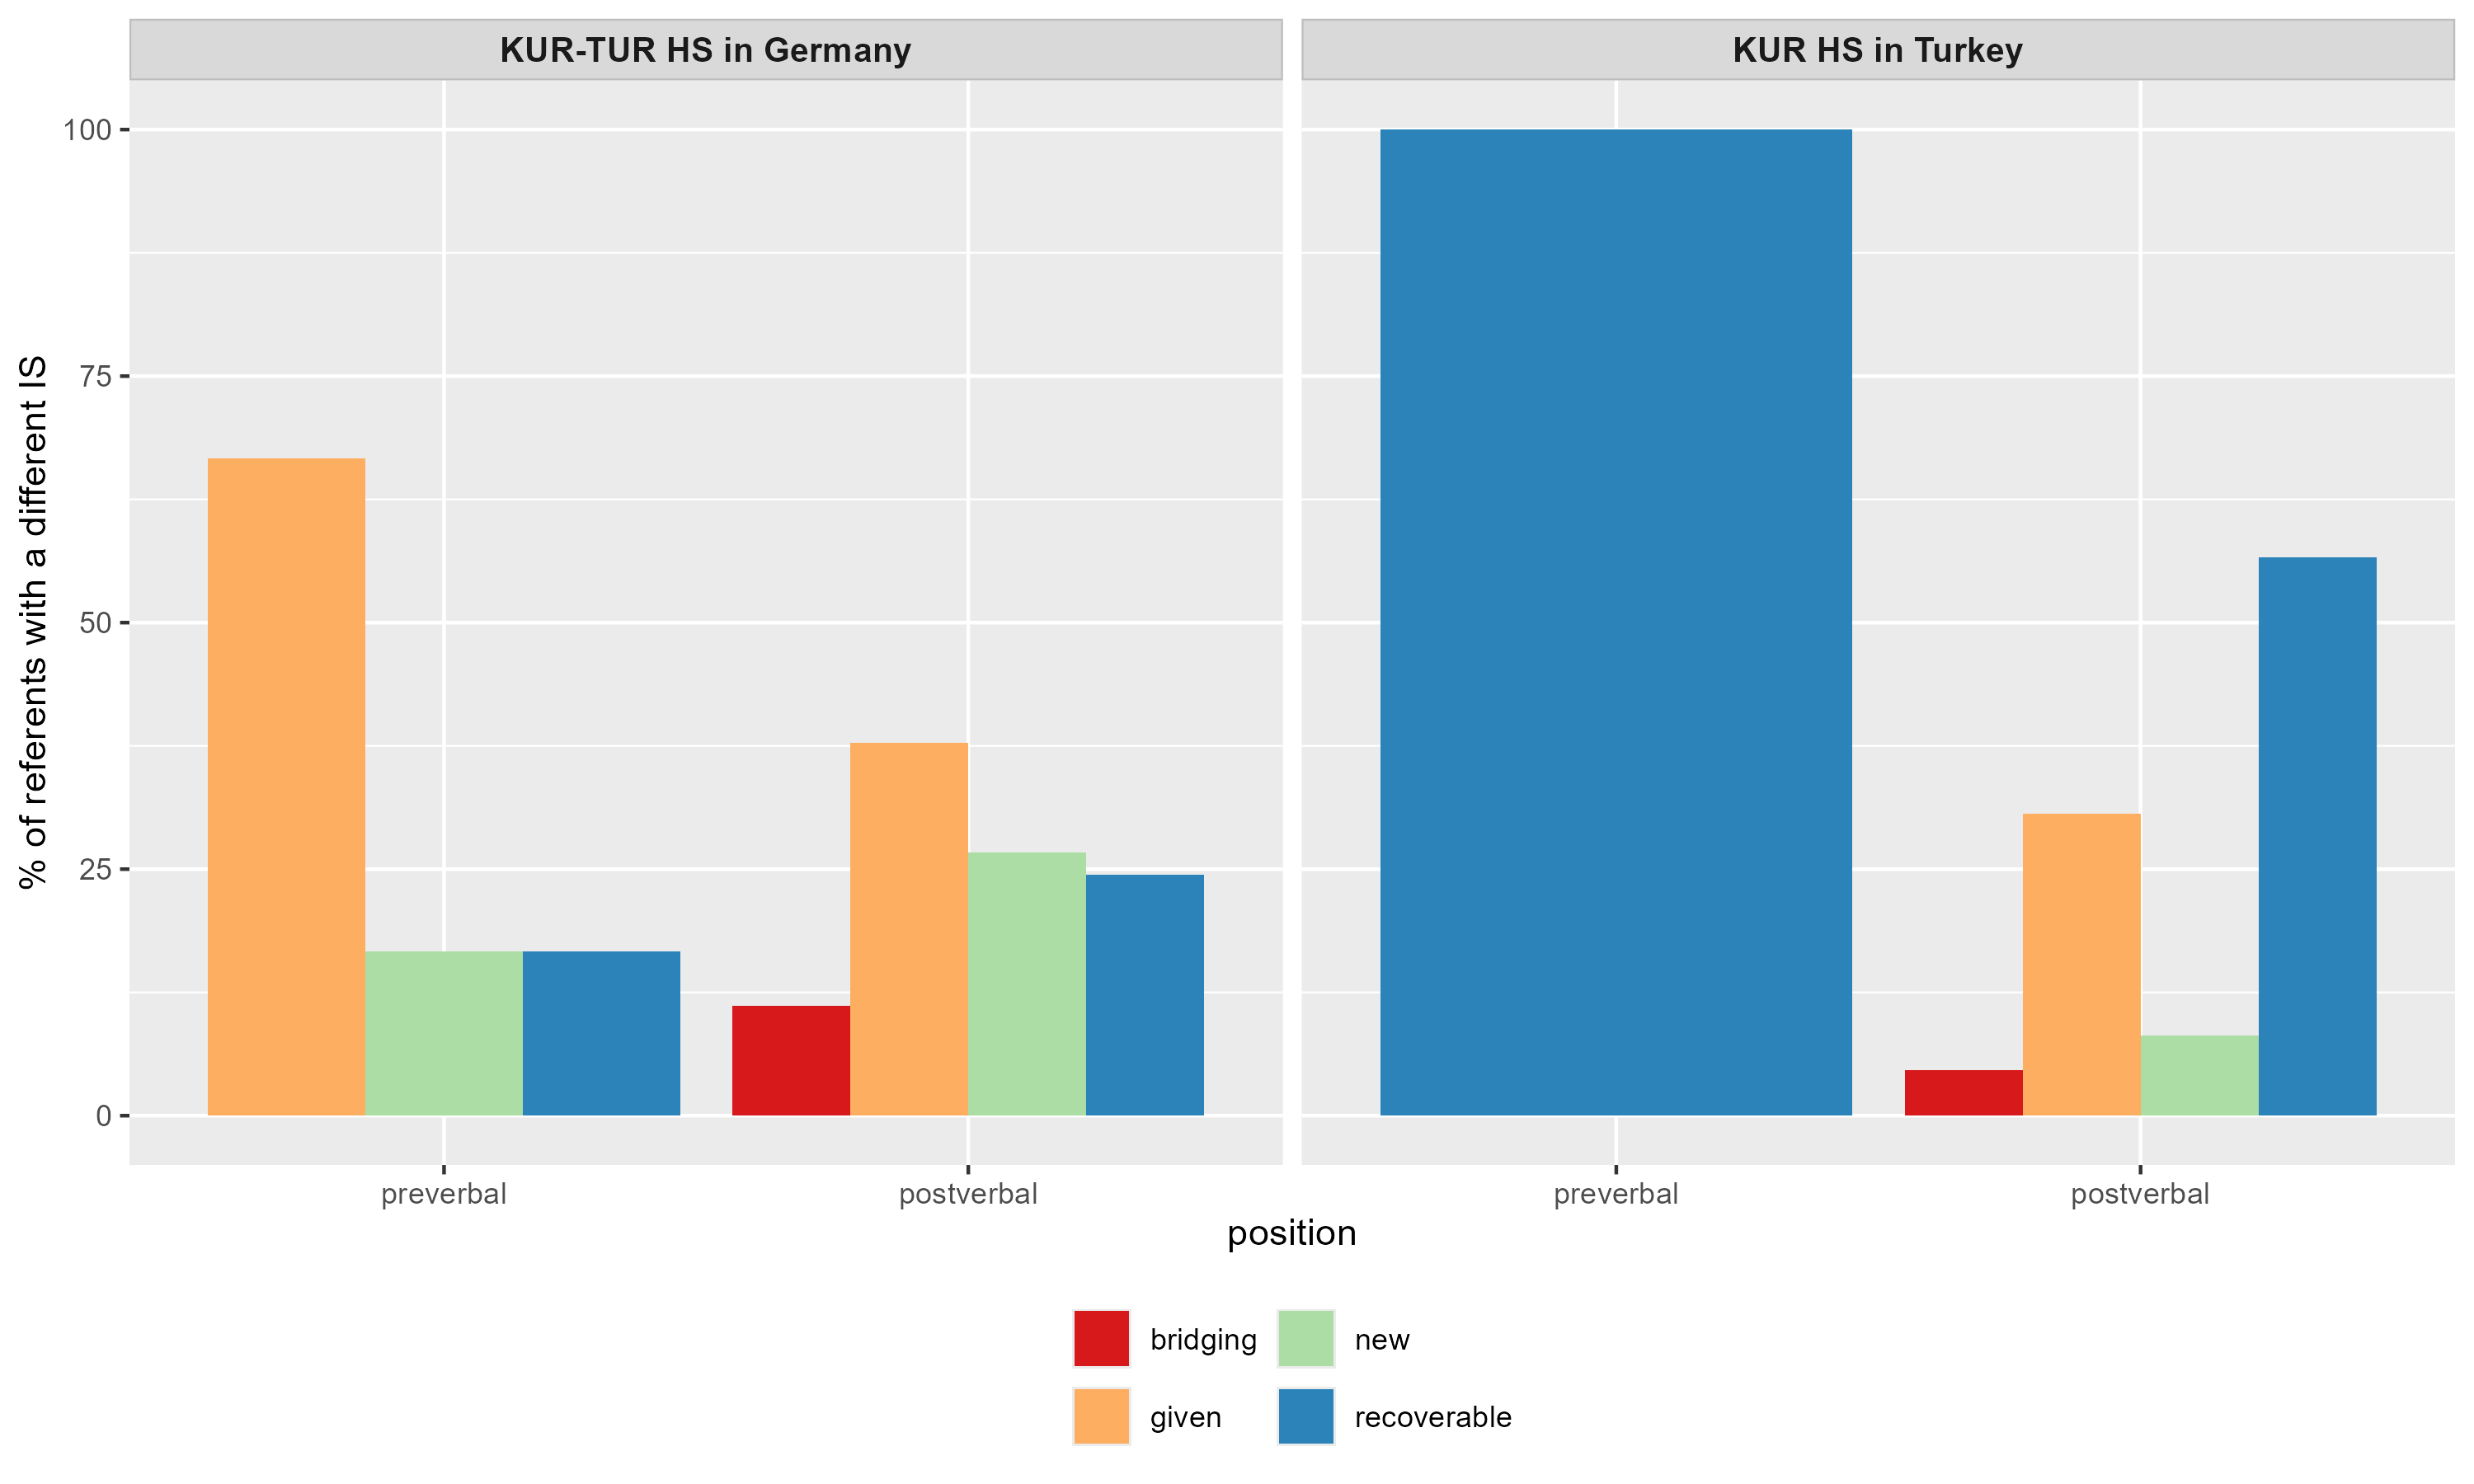
\includegraphics[width=\textwidth]{figures/iefremenko-img018.png}
\caption{\label{fig:key:19}Frequency distribution of goal arguments flagged with case or a locational noun according to their information status.}
\end{figure}

\figref{fig:key:19} illustrates the frequency distribution of goal arguments based on their information status, calculated relative to the total number of goal arguments within each speaker group. For noncanonically placed goal arguments flagged with case or a locational noun (i.e., those in the pre-predicate position), all preverbal goals in Turkey are classified as recoverable information (100\%). In contrast, speakers in Germany place 66.67\% of preverbal goals as given, 16.67\% as new, and 16.67\% as recoverable, although the overall number of preverbal goals is low. Regarding post-predicate goals, speakers in Turkey primarily place recoverable goals (56.65\%) and given goals (30.64\%), with smaller proportions of new (8.09\%) and bridging (4.62\%) referents. In Germany, post-predicate goals include given (37.78\%), new (26.67\%), recoverable (24.44\%), and bridging (11.11\%) referents. Taken together, these percentages indicate that information status does not systematically influence whether goals are placed pre- or post-predicatively in either group, as all types of referents can appear in both positions.

Consequently, these findings do not align with those of \citet{Asadpour2021}, and several factors may contribute to this discrepancy. First, as previously mentioned, Asadour's findings are based on a different variety of Kurdish. Additionally, the current data may not be fully suitable for analyzing information status, given that each participant narrated the same story four times in each language, with a 10-15-minute break between formal and informal sessions and a gap of three to seven days between language sessions.

\subsection{Exploring possible factors influencing the position of adpositional goals (excluding locational nouns) in Kurmanji}\label{sec:key:6.3.3}

The following three analyses will focus on adpositional goals, specifically basic prepositions—either alone or in combination with a locational noun—as well as circumpositions and postpositions, while excluding locational nouns. In the dataset, the position of these adpositional goals varies, and the previous research states that the position of adpositional goals is indeed flexible (\citealt{Haig2014, Haig2018}). Thus, this section will examine which variables may influence the placement of adpositional goals of motion in either the pre- or post-predicate position. Similar to the analysis of goals flagged with case or locational nouns, the first step will be to investigate potential differences in the placement of adpositional goals between the groups. Furthermore, the effects of formality and mode on the positioning of adpositional goals will be analyzed, followed by an exploration of the influence of the information status of these goals.

Importantly, previous research has also shown that the placement of adpositional goals differs among various dialects of Kurmanji (\citealt{Haig2014, Haig2018, Gundogdu2019}). However, because the data were collected in Ankara without accounting for dialectical differences, this factor remains unaddressed in the study.

\subsubsection{The effect of the speaker group on the placement of adpositional goals (excluding locational nouns) in Kurmanji.}\label{6.3.3.1}

The findings in \sectref{sec:key:6.3} indicate that adpositional goals can be found in both pre- and post-predicate positions, and their placement does not appear to be influenced by the speaker group or the majority language of the speakers. To statistically verify whether the speaker group affects the use of case-flagged goals in the pre-predicate position, a generalized logistic mixed-effects model was used, following a binomial distribution. In this model, Position (with preverbal coded as 1 and postverbal coded as 0) served as the dependent variable, while Group (comprising Kurmanji speakers in Turkey (Tubi) and Kurmanji speakers in Germany (Debi)) was treated as a fixed effect. Participant was included as a random variable. The results of the regression analysis are summarized in \tabref{tab:key:15}.


\begin{table}\small
\begin{tabularx}{\textwidth}{XYY}
\lsptoprule
\textbf{Random effects:} & & \\
\midrule
\textbf{Groups} & \textbf{Variance} & \textbf{Standard} \textbf{Deviation}\\
Participant (Intercept) & 2.29 & 1.51\\
% \lspbottomrule
\midrule
\end{tabularx}

\begin{tabularx}{\textwidth}{Xrrrr}
% \lsptoprule
\textbf{Fixed effects:} & & & & \\
\midrule
\textbf{Fixed} \textbf{effect} & \textbf{Estimate} & \textbf{Std. Error} & \textbf{z-value}  & \textbf{\textit{p}-value}\\
Intercept & -0.90 & 0.97 & -0.94 & .35\\
Group (Tubi) & 0.97 & 1.08 & 0.90 & .37\\
\lspbottomrule
\end{tabularx}
\caption{\label{tab:key:15}Regression table for glmer with the dependent variable Position and the independent variable Group.}
\end{table}

As anticipated, the results of the regression analysis indicate that the speaker group has no significant effect on goal position.

\subsubsection{The effect of formality and mode on the placement of adpositional goals (excluding locational nouns) in Kurmanji.}\label{sec:key:6.3.3.2}

To determine whether formality and mode influence the position of adpositional goals, a binomial generalized linear mixed-effects model was used to assess the effects of these factors on the placement of adpositional goals. In this model, the dependent variable is the Position of Adpositional Goals (preverbal coded as 0 and postverbal coded as 1), while the independent variables include the interaction between Formality (formal vs. informal) and Mode (spoken vs. written). The model also accounted for individual variation within the data by incuding the variable Participant as a random variable. An overview of the regression results can be found in \tabref{tab:key:16}.

\begin{table}\small
\begin{tabularx}{\textwidth}{XYY}
\lsptoprule
\textbf{Random effects:} & & \\
\midrule
\textbf{Groups} & \textbf{Variance} & \textbf{Standard} \textbf{Deviation}\\
Participant (Intercept) & 3.07 & 1.75\\
% \lspbottomrule
\midrule
\end{tabularx}

\begin{tabularx}{\textwidth}{Xrrrr}
% \lsptoprule
\textbf{Fixed effects:} & & & & \\
\midrule
\textbf{Fixed} \textbf{effect} & \textbf{Estimate} & \textbf{Std. Error} & \textbf{z-value}  & \textbf{\textit{p}-value}\\
Intercept & {}-0.87 & 0.60 & {}-1.44 & .14\\
Formality (informal) & 1.26 & 0.62 & 2.02 & $.43^{*}$\\
Mode (written) & 0.53 & 0.63 & 0.85 & .39\\
\lspbottomrule
\end{tabularx}
\caption{\label{tab:key:16}Regression table for binomial glmer with the dependent variable Position of ADP Flagged Goals and the independent variables Formality and Mode.}
\end{table}

\newpage
Formality: Formality is a binary independent variable assigned the levels formal and informal in my study. As seen in \tabref{tab:key:16}, informality significantly facilitates the placement of adpositional goals of motion in the post-predicate position. This is also demonstrated in \figref{fig:key:20}.

Mode: Mode is a binary independent variable with the levels spoken and written. The model shows no reliable or significant effect of Mode.

\begin{figure}[t]
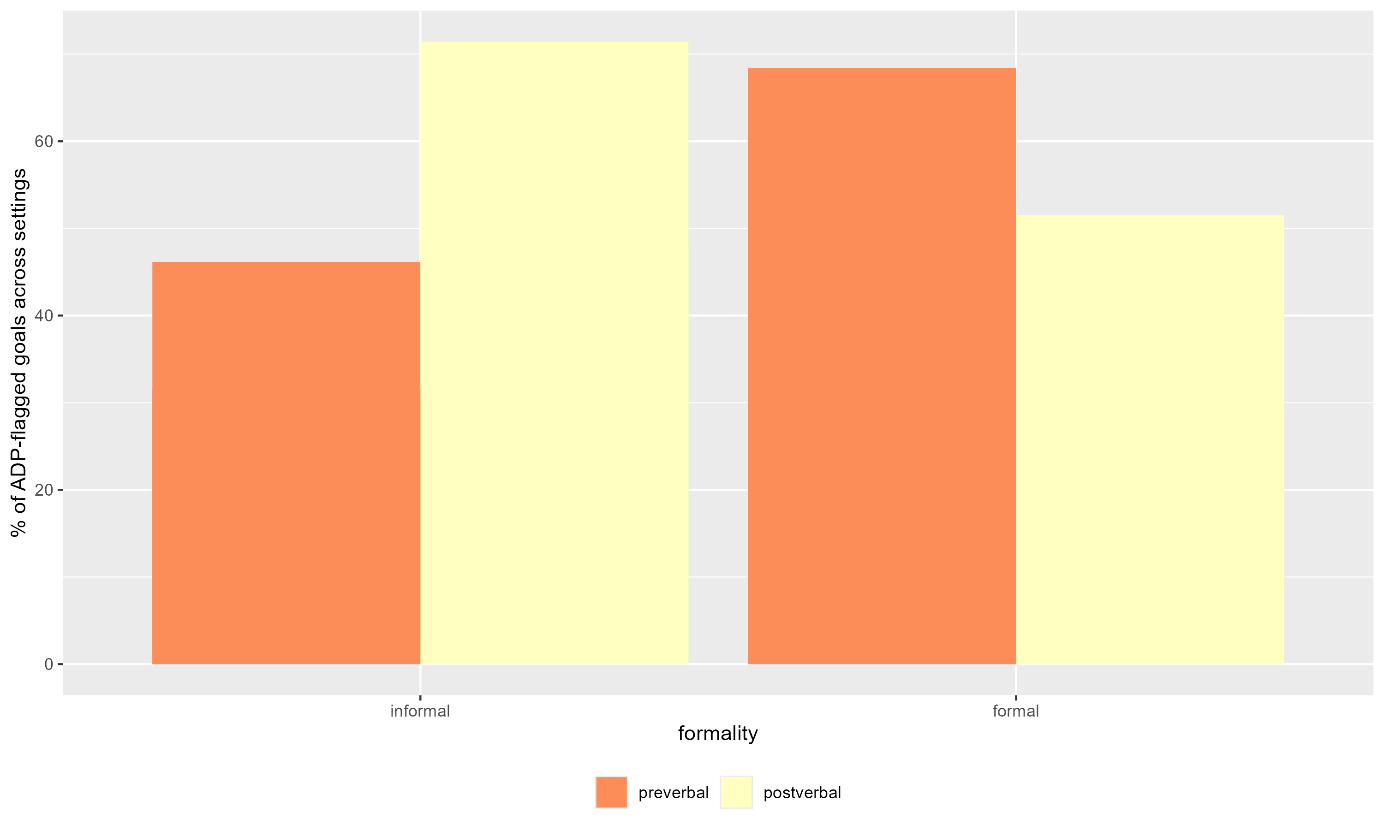
\includegraphics[width=\textwidth]{figures/iefremenko-img019.png}
\caption{\label{fig:key:20}Frequency distribution of ADP-flagged goals of motion in the pre- and post-predicate position across formal and informal settings.}
\end{figure}

Thus, the regression analysis showed the effect of formality: while the post-predicate goals are more likely to occur in the informal data, the pre-predicate goals were more likely to be used in the formal communicative situations.

\subsubsection{The effect of information structure on the placement of adpositional goals (excluding locational nouns)}\label{sec:key:6.3.3.3}

Next, the role of information structure in the placement of adpositional goals will be explored. Similar to the analysis of goals of motion flagged with case or a locational noun, the information status of the adpositional goal arguments has been annotated, differentiating between new, given, bridging, and recoverable statuses. The results of this analysis are presented in \figref{fig:key:21}.

\begin{figure}
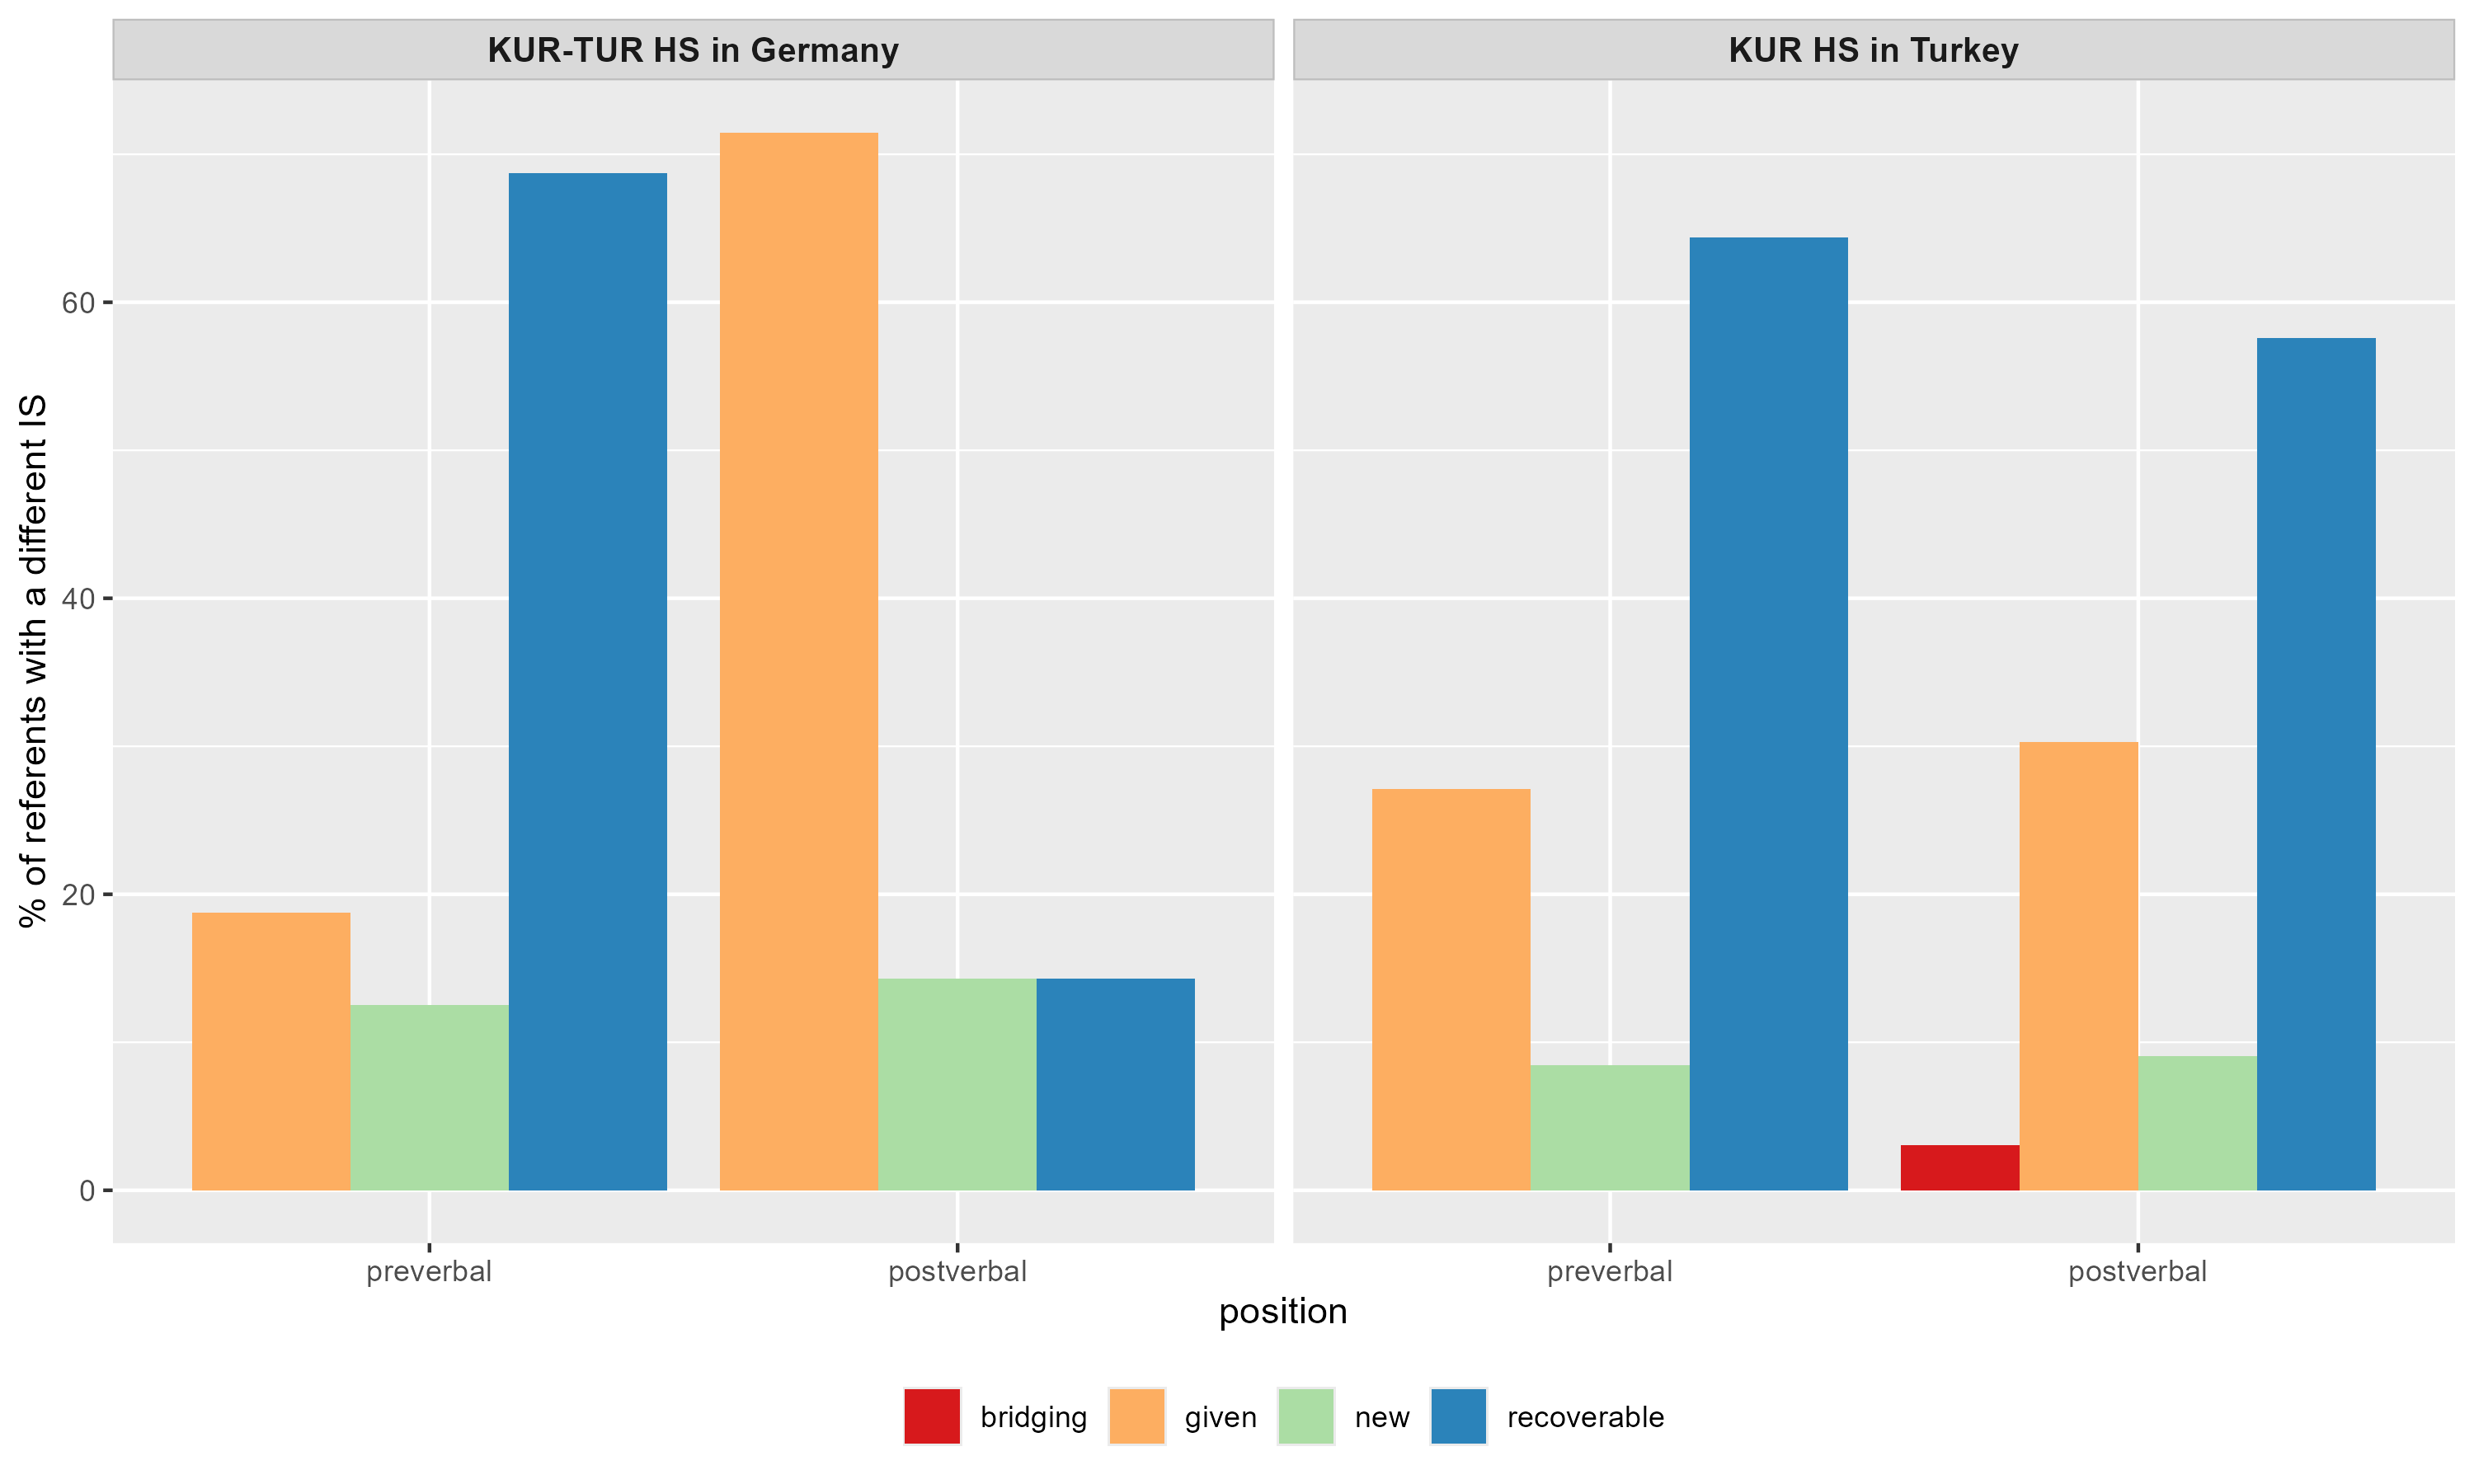
\includegraphics[width=\textwidth]{figures/iefremenko-img020.png}
\caption{\label{fig:key:21} Frequency distribution of goal arguments flagged with an adposition according to their information status.}
\end{figure}

\figref{fig:key:21} illustrates that recoverable and given goals are the most frequent in the dataset, although their placement varies by speaker group. In Turkey, postverbal goals are most often recoverable (57.6\%), followed by given (30.3\%) and new referents (9.1\%), while bridging referents are virtually absent (3.0\%). In the preverbal position, recoverable referents are again the most frequent (64.4\%), with given (27.1\%) and new (8.5\%) referents occurring less often. This indicates a relatively balanced distribution across positions, with recoverable information dominating in both. In Germany, postverbal goals are predominantly given (71.4\%), with recoverable and new referents occurring much less frequently (14.3\% each). In contrast, preverbal goals are mostly recoverable (68.8\%), followed by given (18.8\%) and new (12.5\%) referents. Hence, there is no clear effect of information status on the placement of adpositional goals of motion.

\subsection{Interim summary}\label{sec:key:6.3.4}

To summarize the findings on goals of motion in Kurmanji, results indicate that goals of motion flagged with case or an adposition can appear in both pre- and post-predicate positions, though the post-predicate position is generally preferred. Previous research (\citealt{Haig2014, Gundogdu2019}) suggests that goals of motion flagged with case or a locational noun are restricted to the post-predicate position. However, the data analyzed here include instances where such goals also appear in the pre-predicate position.

Regression analyses revealed no correlation between group, formality and mode, and the placement of case-flagged goals or those marked with locational nouns. Besides, information structure does not seem to play a role of the position of these constituents. However, qualitative analysis showed that in the Kurmanji data from Turkey, all pre-predicate occurrences of case-flagged goals appear in the same construction \textit{erdê ketin} (‘to fall on the ground’), whereas the data from Germany exhibit greater variation in verb usage with case-flagged arguments in the pre-predicate position. Similarly, in the data from Turkey, locational nouns in the pre-predicate position predominantly occur in the construction \textit{hemberî rê} (‘across the road’), while no such pattern emerges in the data from Germany.

Regarding goals flagged with adpositions, previous research (\citealt{Haig2014, Gundogdu2019}) suggests that their position is more flexible compared to goals of motion flagged with case or locational nouns. The present findings confirm this variability. Notably, regression analysis identified formality as a significant predictor for the placement of adpositional goals: while the post-predicate position is more frequent in the informal situations, the pre-predicate position is preferred in the formal settings.

\subsection{Addressees of verbs of speech}\label{sec:key:6.3.5}

The focus now shifts to the second most frequent type of goals in the data: addressees of verbs of speech. Similar to goals of motion in Kurmanji, addressees of verbs of speech can be flagged with the oblique case (see example \ref{ex:key:77} or an adposition (see example \ref{ex:key:78}).


\ea \label{ex:key:77} Kurmanji, TUbi10MK\_fwK \\
\gll Ez    di-xwaz-im   agahî     bi-di-m     we \\
\textsc{1sg.nom}  \textsc{prs-}want-\textsc{1sg}  news    \textsc{subj-}give-\textsc{1sg}    you.\textsc{2pl}\\
\glt ‘I want to inform you.’ 
\z

\ea%76
  \label{ex:key:78} Kurmanji, TUbi05MK\_fwK \\
\gll Mi     go     e  ji   te     ra   bi-bêj-im \\
\textsc{1sg.obl}    say\textsc{.pst}    hm  to  \textsc{2sg.obl}    \textsc{circ}  \textsc{subj}-say-\textsc{1sg}  \\
\glt ‘I said, I am telling to you.’  
  \z

As with goals of motion, the position of addressee arguments depends on the type of flagging and the dialect. According to \citet{Gundogdu2019}, case-flagged goals always appear post-predicate (as in example \ref{ex:key:77}), while adpositional addressees are typically placed in the pre-predicate position (as in example \ref{ex:key:78}). However, regional variation influences both the position and the types of adpositions used in Kurmanji (\citealt{Haig2014}, \citealt{Haig2022}). In southeastern dialects, addressees are case-flagged and post-predicate, whereas in northern dialects, they are primarily adpositional and appear pre-predicatively. Additionally, different northern dialects exhibit distinct preferences for adpositional flagging: in the Northern dialect (e.g., Muş), speakers predominantly use the circumposition \textit{ji…ra} (‘to’), while in the Northwestern dialect (e.g., Malatya), the postposition \textit{…ra} (‘to’) is preferred (\citealt{Gundogdu2019}). Notably, addressees flagged with a circumposition cannot be placed post-predicatively and must always appear in the pre-predicate position (\citealt{Gundogdu2019}).

The frequency distribution of addressees flagged with the oblique case or an adposition in either the pre- or post-predicate position is presented in \figref{fig:key:22}.

\begin{figure}
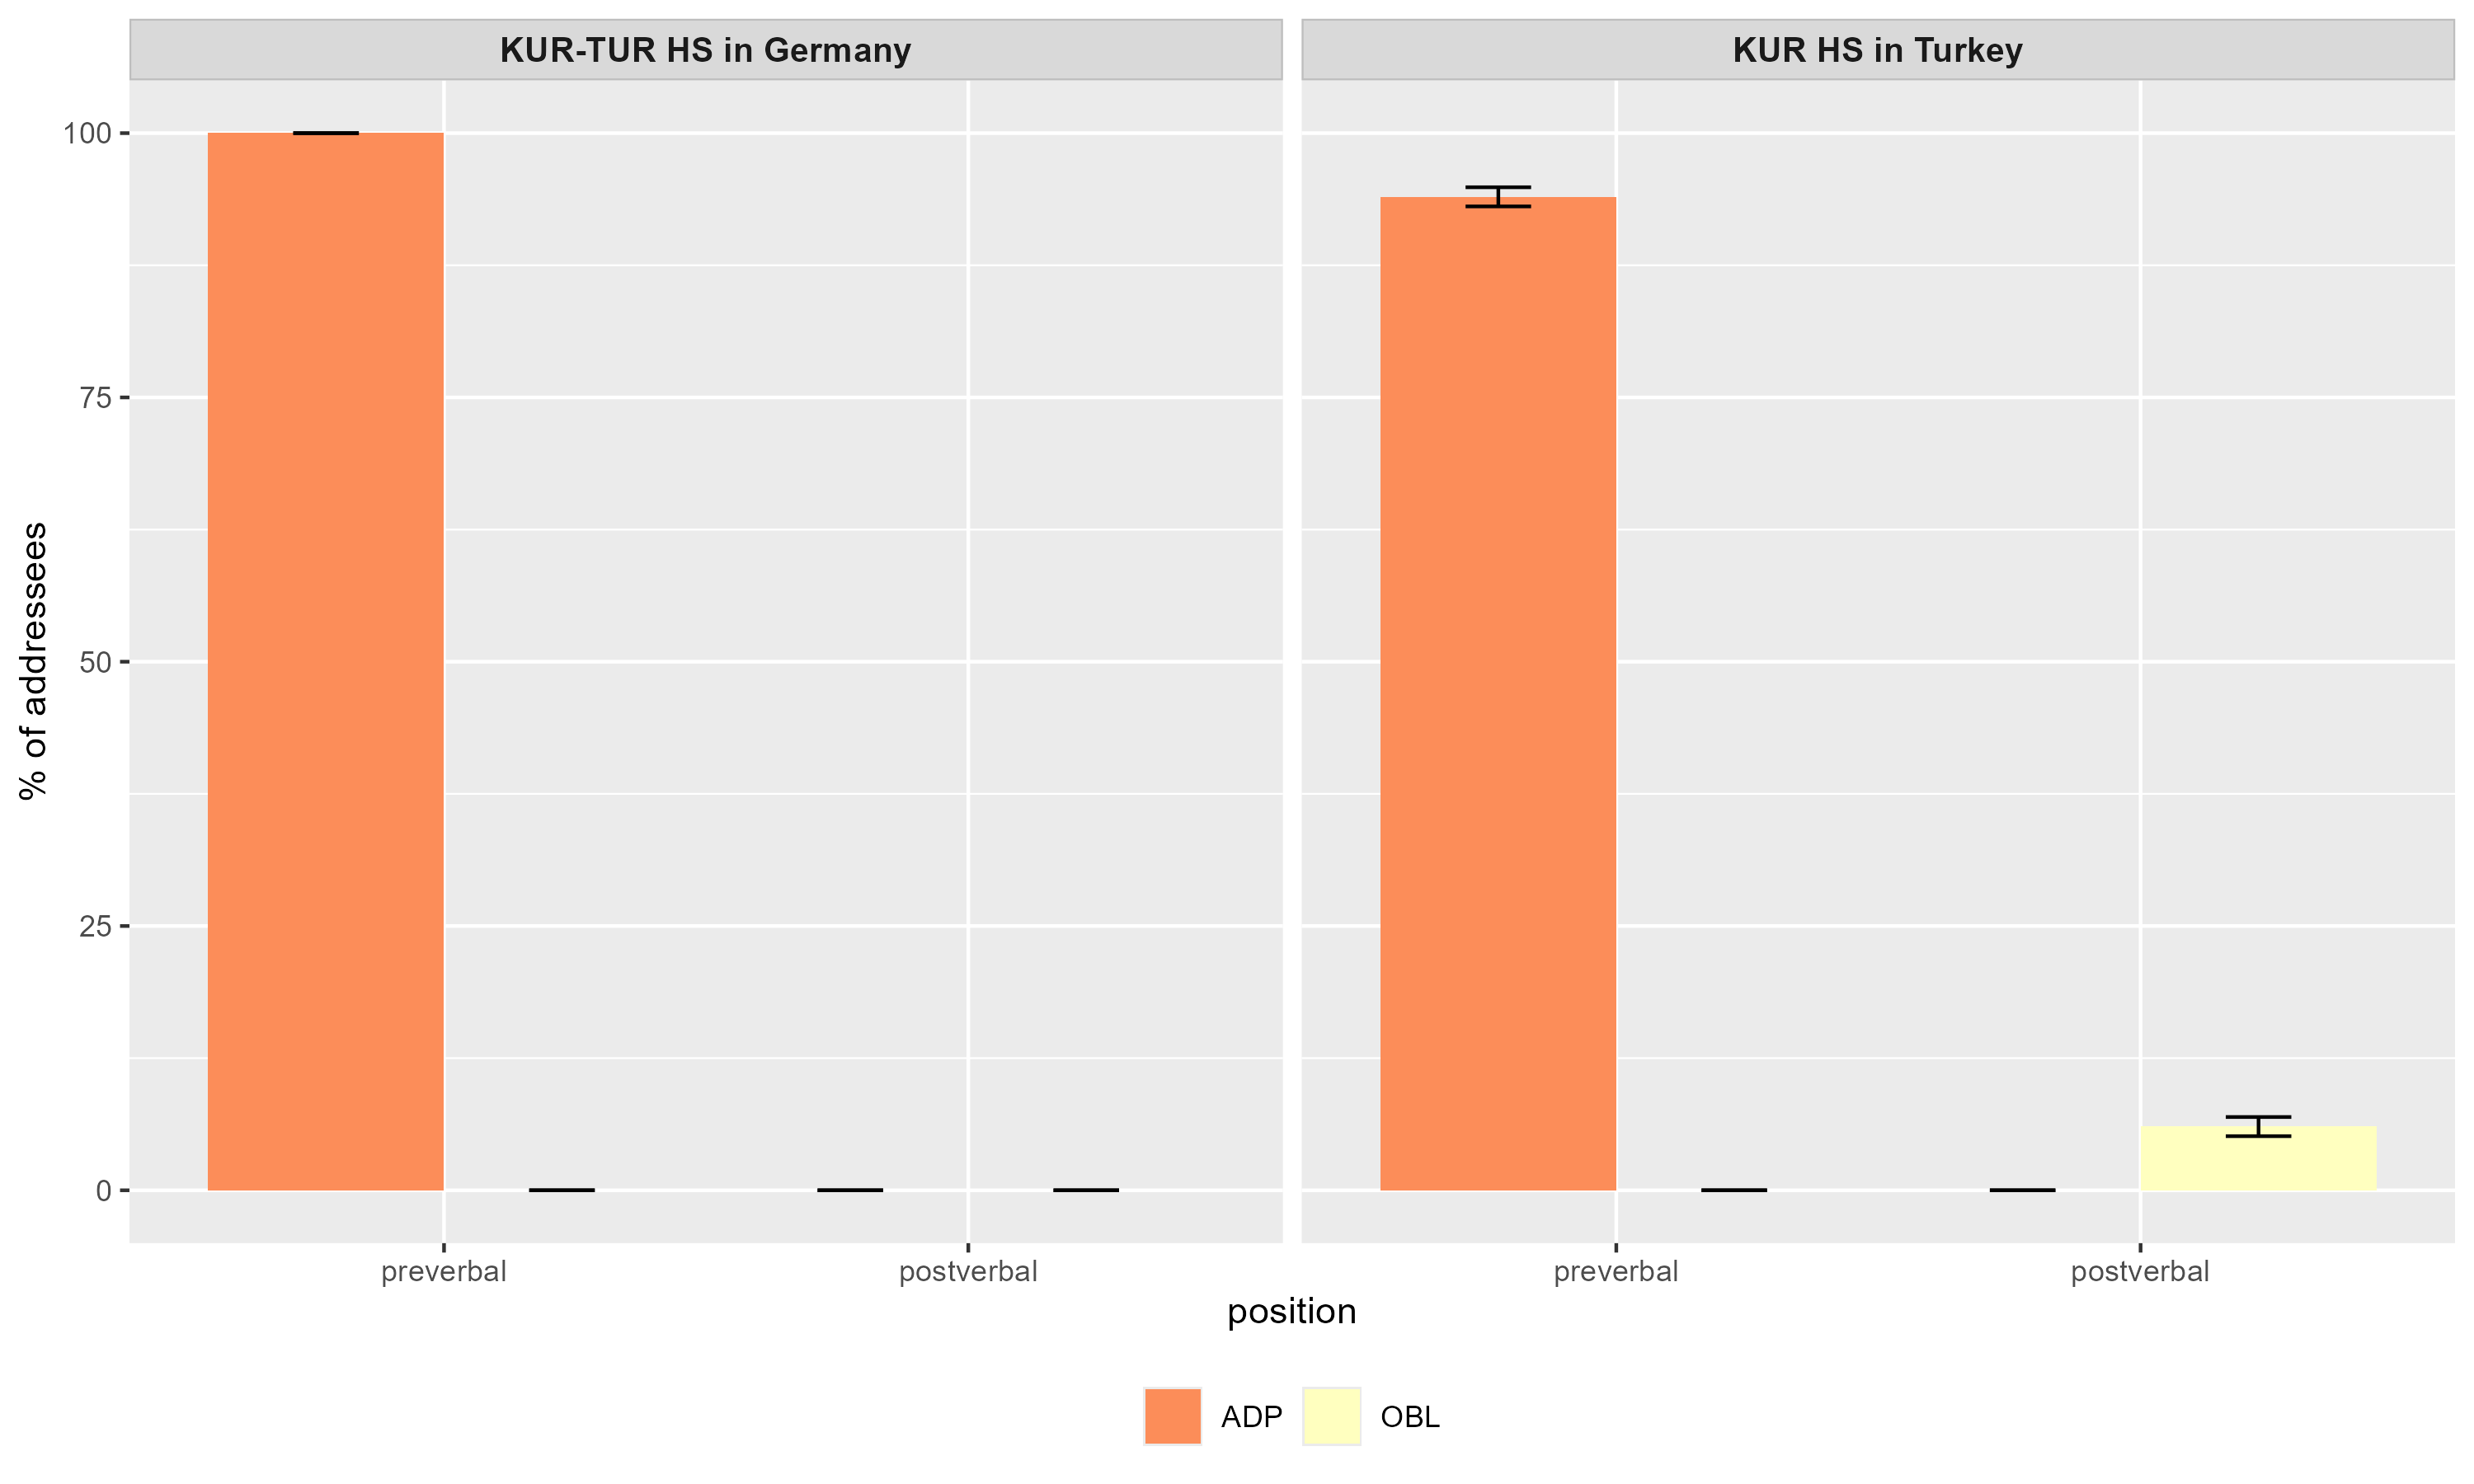
\includegraphics[width=\textwidth]{figures/iefremenko-img021.png}
\caption{\label{fig:key:22}Frequency distribution of addressees flagged with the oblique case or an adposition in the pre- and post-predicate position (in \%) in relation to the total number of addressees.}
\end{figure}

As mentioned in \sectref{sec:key:6.3}, the video shown to the participants elicited fewer addressees compared to goals of motion. The data includes 24 instances of arguments of verbs of speech from Kurmanji speakers in Turkey and only three instances from Kurmanji speakers in Germany. Therefore, the frequencies in the plot should be interpreted with caution.

The left-hand plot in \figref{fig:key:22} illustrates that all three examples from Kurmanji-Turkish HS in Germany are flagged with an adposition and appear in the pre-predicate position. Similarly, the right-hand plot shows that speakers in Turkey also predominantly flag addressees with an adposition and place them preverbally, aligning with previous research (\citealt{Gundogdu2019, Haig2022}).

\tabref{tab:key:17} presents the absolute number of addressees flagged with either case or an adposition in the pre- or post-predicate position. Additionally, the table provides information on the type of adposition used, distinguishing between the circumposition \textit{ji…ra} and the postposition \textit{…re/ra}.

\begin{table}
\begin{tabularx}{\textwidth}{llYYY}
\lsptoprule
Country & Position & OBL flagged & Flagged with circumposition
(\textit{ji…re/ra}) & Flagged with a postposition (\textit{re/ra})\\
\midrule
Turkey & pre- & - & 16 & 5\\
& post- & 3 & - & -\\
Germany & pre- & - & 1 & 2\\
& post- & - & - & -\\
\lspbottomrule
\end{tabularx}
\caption{\label{tab:key:17} The absolute number of addressees flagged with the help of oblique case or an adposition placed in the pre- or post-predicate position.}
\end{table}

\tabref{tab:key:17} indicates that speakers in Turkey predominantly flag addressees with the circumposition \textit{ji…ra} and place them in the pre-predicate position. However, in both country groups, some addressees are flagged using the postposition \textit{re/ra}—five instances in the data from Turkey and two from Germany—all of which occur in the pre-predicate position.

In addition to addressees marked with a circumposition or postposition, three instances of case-flagged addressees appear in the data. As previously mentioned, the only canonical position for case-flagged goals is post-predicate. Consistently, all three examples in the data follow this pattern (see example 79).

\ea \label{ex:key:79} Kurmanji, TUbi11FK\_iwK \\
\gll cane pesiye   di-xwaz-im     silav-ek   bi-di-m     te  \\
dear  {}  \textsc{prs-}want-\textsc{1sg}    hello-\textsc{indf}  \textsc{subj-}give-\textsc{1sg}    you.\textsc{2pl} \\
\glt ‘My dear, I would like to say hello to you’. 
\z

Due to the limited number of addressees in the data, it is not possible to run statistical models to examine correlations between variables such as speaker group, formality, mode, or information status and the position of addressees.

However, the quantitative analysis indicates that Kurmanji speakers in both Turkey and Germany follow the word order patterns observed in previous studies. Case-flagged goals consistently appear in the immediate post-predicate position, while adpositional goals are placed pre-predicatively. These findings confirm that the position of addressees is primarily determined by the type of flagging.

Regarding the effect of formality and mode, the qualitative analysis of the data revealed that addressees appear in both pre- and post-predicate positions across all communicative situations. This suggests that formality and mode do not influence the positioning of addressees. Additionally, all addressees in the data are expressed using second-person singular and plural pronouns in contexts such as "I’d like to tell you about...," which precludes an analysis of information status for addressees.

\subsection{Non-goal constituents in the post-predicate position}\label{sec:key:6.3.6}

As previously demonstrated, Kurmanji is an OVX language, with X reserved for goal of motion, addressees of verbs of speech and recipients of verbs of transfer. However, as illustrated earlier in this chapter and shown again in \figref{fig:key:23} for convenience, there are also other constituents in the data placed in the post-predicate position.

\begin{figure}
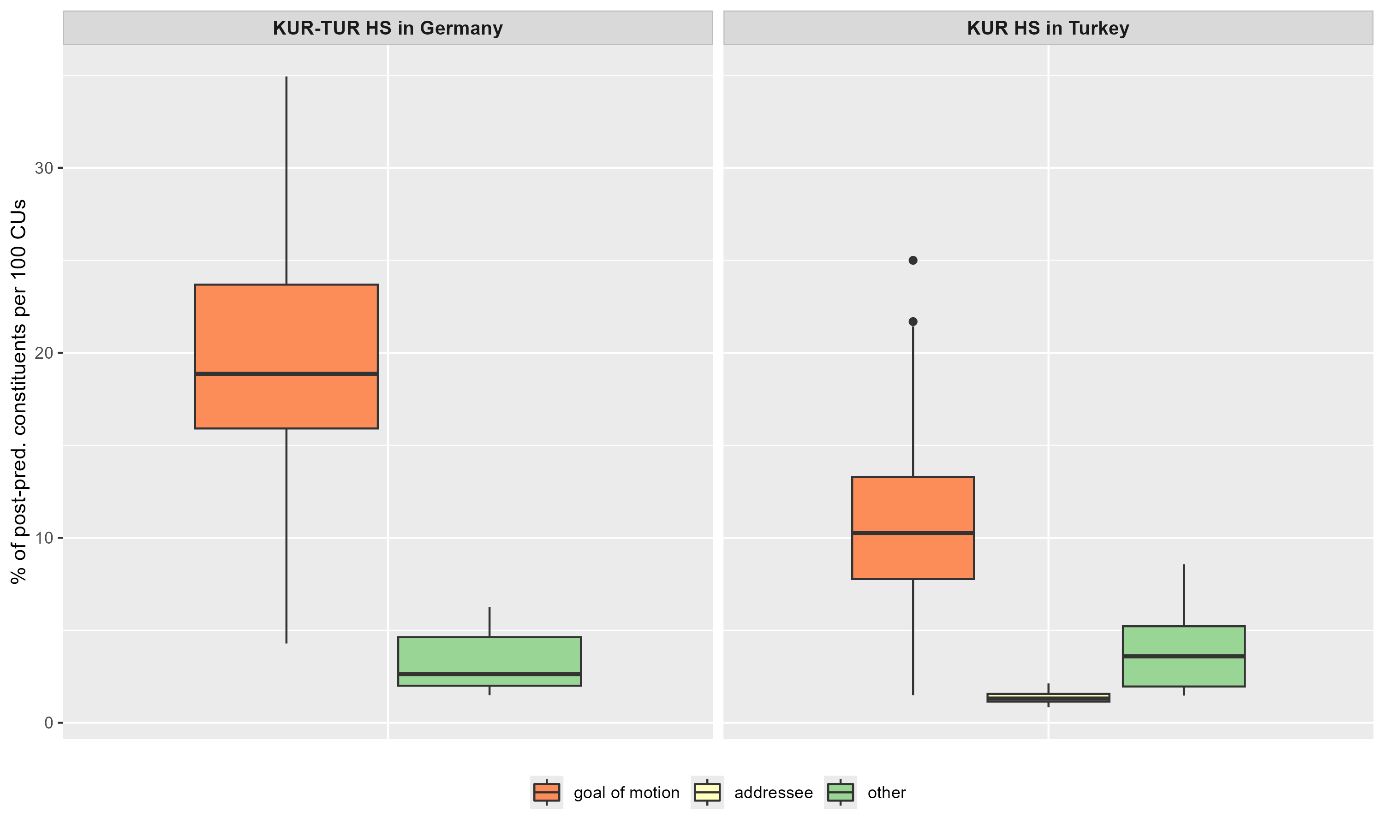
\includegraphics[width=\textwidth]{figures/iefremenko-img015.png}
\caption{\label{fig:key:23}Types of post-predicate structures in Kurmanji in two country groups.}
\end{figure}

\figref{fig:key:23} illustrates that approximately 3\% (n=15) of all the CUs in the data from Germany and about 4\% (n=55) of the CUs in the data from Turkey contain non-goal constituents in the post-predicate position. To determine whether one group shows a statistically significant tendency to place non-goal constituents in the post-predicate position compared to the other, a linear regression model was conducted, with the Percentage of Non-Goal Constituents in the Post-Predicate Position as the dependent variable and Group as the fixed effect.

\begin{table}
\begin{tabularx}{\textwidth}{XYYYY}
\lsptoprule
\textbf{Fixed effect} & \textbf{Estimate} & \textbf{Std. Error} & \textbf{t-value}  & \textbf{p-value}\\
\midrule
(Intercept) & 3.29 & 0.74 & 4.40 & $.0001^{***}$\\
Group (Tubi) & 0.71 & 0.86 & 0.82 & .41 \\
\lspbottomrule
\end{tabularx}
\caption{\label{tab:key:18}Regression table for LM with a dependent variable Percentage of Non-Goal Constituents in the Post-Predicate Position and an independent variable Country.}
\end{table}

\largerpage
Group: The variable Group is treated as a binary variable with two levels: Germany and Turkey. The model did not reveal any significant effects related to the country variable.

The linear model indicated that there are no significant differences between the groups regarding the placement of non-goal constituents in the post-predicate position. Therefore, the observed higher frequency of post-predicate structures in Germany, as discussed in \sectref{sec:key:6.1}, cannot be attributed to a greater number of non-goal constituents used by speakers in Germany compared to those in Turkey.

To further explore the characteristics of non-goal constituents placed in the post-predicate position in Kurmanji and to understand the source of the occurrence of such structures, the following analysis will examine various features, including phonological weight, types of constituents, and their semantic roles.

\subsubsection{Weight of non-goal post-predicate constituents in Kurmanji}\label{sec:key:6.3.6.1}

The analysis will begin with the weight of non-goal constituents in the post-predicate position. It is anticipated that speakers will preferentially place longer segments in this position, as this strategy may help mitigate the limitations in working memory capacity experienced by both speakers and listeners.

Following \citep{Haignforth}, four types of weight for non-goal post-predicate constituents will be identified, paralleling the analysis of post-predicate constituents in Turkish described in Section \ref{sec:key:5.3.1}. Post-positive constituents are italicized for clarity.

\begin{itemize}
\item Weight 1: a single phonological word.

\ea
  \label{ex:key:80} Kurmanji, TUbi15MK\_isK \\
     \gll Ez     ji   wir   çû-m     \textit{yanî}\\
\textsc{1sg.nom}  from  there  go\textsc{.pst-1sg}  well\\
\glt ‘I was going from there yani.’
  \z


\item{Weight 2:} two phonological words.

\ea%79
  \label{ex:key:81} Kurmanji, TUbi30FK\_isK \\
     \gll û:   kûçik   jî   tirsîya     \textit{ji}   \textit{top-ê} \\
and  dog  also  scare\textsc{.pst.3sg}  from  ball-\textsc{obl}  \\
\glt ‘And the dog got scared of the ball.’ 
  \z


\item{Weight 3:} three phonological words.

\ea%80
  \label{ex:key:82} Kurmanji, TUbi26MK\_isK \\
     \gll Mêr   û   jin-ek-î     ji   wê   da   di-hat-in \textit{tevî}     \textit{sebî-yê}     \textit{xwe}\\
man  and  woman-\textsc{indf-obl.f}  from  her  \textsc{post}  \textsc{prs}-come-\textsc{3pl} together  baby-\textsc{ez}  \textsc{refl}\\
\glt ‘A man and a woman were coming from her with their child.’  
  \z


\item{Weight 4:} four or more phonological words.

\ea%81
  \label{ex:key:83} Kurmanji, DEtr10FK\_iwK \\
     \gll Çink-ek   hawo     \textit{ba}   \textit{guddik}, \textit{ba}   \textit{torb-ok}  \textit{sew}\\
woman\textsc{-indf}  have\textsc{.pst.3sg}  with  dog   with  bag-\textsc{indf}  apple\\
\glt ‘There was a woman with a dog, with a bag of apples.’ 
  \z

\end{itemize}

Thus, in essence, every element can contribute to the overall weight of a constituent. Notably, unlike Turkish, Kurmanji frequently uses adpositions that add additional weight to post-predicate structures. However, adpositions comprising two or three elements, such as circumpositions, are considered as constituents with a weight of 1. For example, in \REF{ex:key:82}, the post-predicate structure \textit{di bûyerê de} (‘in the incident’) is assigned a weight of two phonological words, as the circumposition \textit{di…de} is treated as a single element in this analysis.

\ea%82
  \label{ex:key:84} Kurmanji, TUbi17FK\_fsK \\
        \gll Lê   kesek     birîndar   ne-bû     di   buyer-ê   de\\
but  somebody  injured    \textsc{neg}-be\textsc{.pst.3sg} \textsc{circ}  accident-\textsc{obl.f} \textsc{circ}\\
\glt ‘But no one was injured in the incident.’ 
  \z

The results of the analysis of the weight of non-goal post-predicate structures in Kurmanji are presented in \figref{fig:key:24}.

\begin{figure}[b]
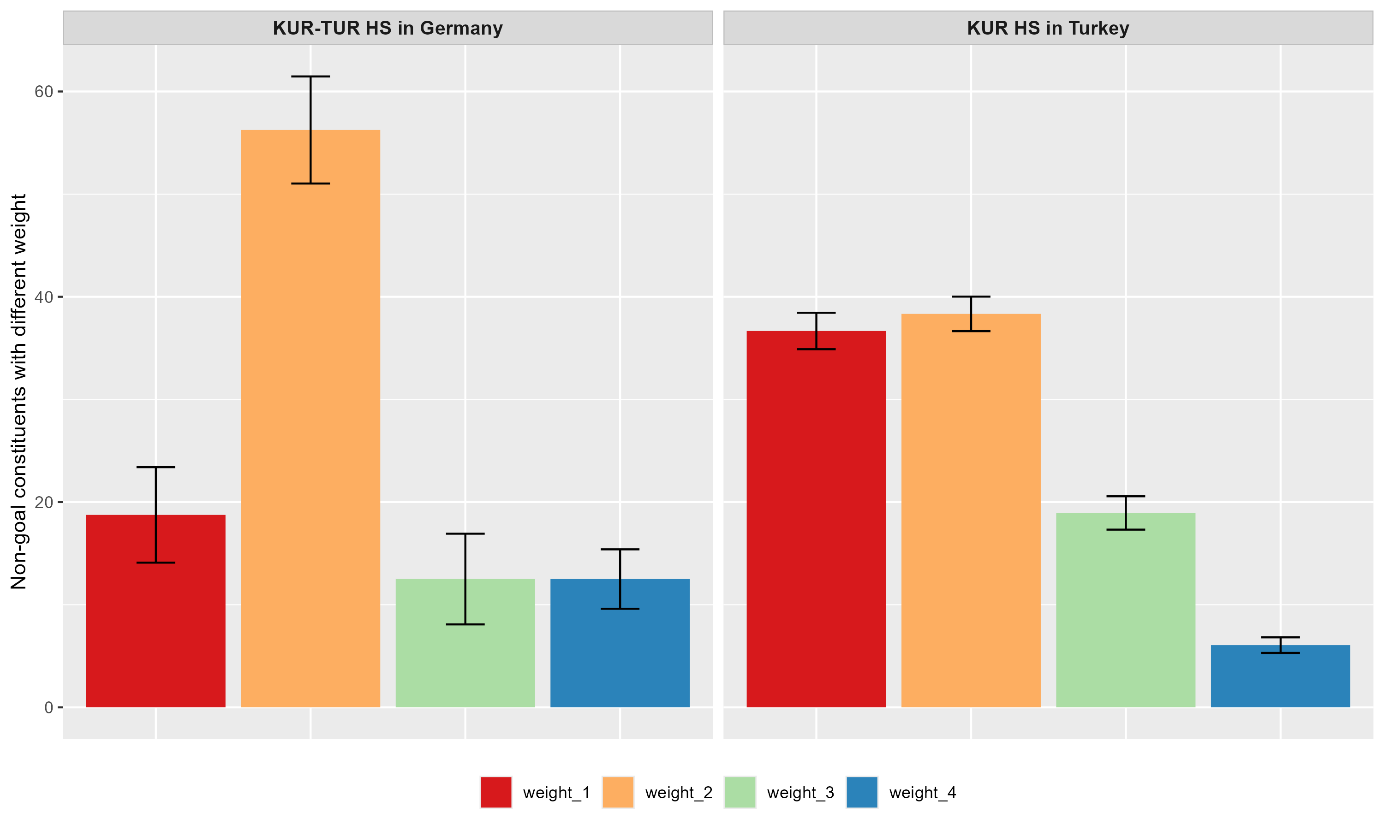
\includegraphics[width=\textwidth]{figures/iefremenko-img022.png}
\caption{\label{fig:key:24}Frequency distribution of non-goal post-predicate structures with different weight calculated in relation to the total number of non-goal post-predicate structures in each group.}
\end{figure}

\figref{fig:key:24} illustrates the frequency distribution of non-goal post-predicate structures with varying weights, calculated in relation to the total number of non-goal post-predicate structures within each speaker group. Error bars represent the standard error. The analysis reveals that speakers in Germany predominantly use post-predicate structures consisting of two elements, whereas speakers in Turkey exhibit a roughly even distribution of examples between post-predicate structures composed of one and two phonological words.

It is important to note, however, that the frequency distribution depicted in \figref{fig:key:24} is based on a very limited number of examples, particularly within the German group. Consequently, no statistical tests will be conducted for this or the subsequent analyses of non-goal constituents.

\subsubsection{Types of non-goal post-predicate structures in Kurmanji}\label{sec:key:6.3.6.2}

The following section will focus on the types of non-goal constituents previously discussed. The categorization of these types is based on the classification used for post-predicate structures in Turkish (see \sectref{sec:key:5.3.2}), as outlined by \citet{SchroederEtAl2024}. Accordingly, three types of constituents will be identified:

\begin{itemize}
\item Type 1: nominal constituents


\ea \label{ex:key:85} Kurmanji, TUbi17FK\_fsK \\
\gll Lê   kesek     birîndar   ne-bû       \textit{di}   \textit{buyer-ê}   \textit{de}\\
but  somebody  injured    \textsc{neg}-be\textsc{.pst.3sg}  in  accident-\textsc{obl}  \textsc{circ}\\
\glt ‘But no one was injured in the incident.’ 
  \z


\item Type 2: adverbs


\ea\label{ex:key:86} Kurmanji, TUbi18MK\_fsK \\
\gll Arabay fîren   kir     \textit{niha}\\
car  break  do\textsc{.pst.3sg}  now\\
\glt ‘The car braked now.’ 
  \z


\item Type 3: discourse markers


\ea \label{ex:key:87} Kurmanji, TUbi15MK\_isK \\
\gll Ez   ji   wir   çû-m     \textit{yanî}\\
I  from  there  go\textsc{.pst-1sg}  well\\
\glt ‘I was going from there yani’ 
  \z

\end{itemize}

If a post-predicate structure included two or more types, each type was calculated separately. The analysis of the different types of non-goal constituents is presented in \figref{fig:key:25}.

\begin{figure}
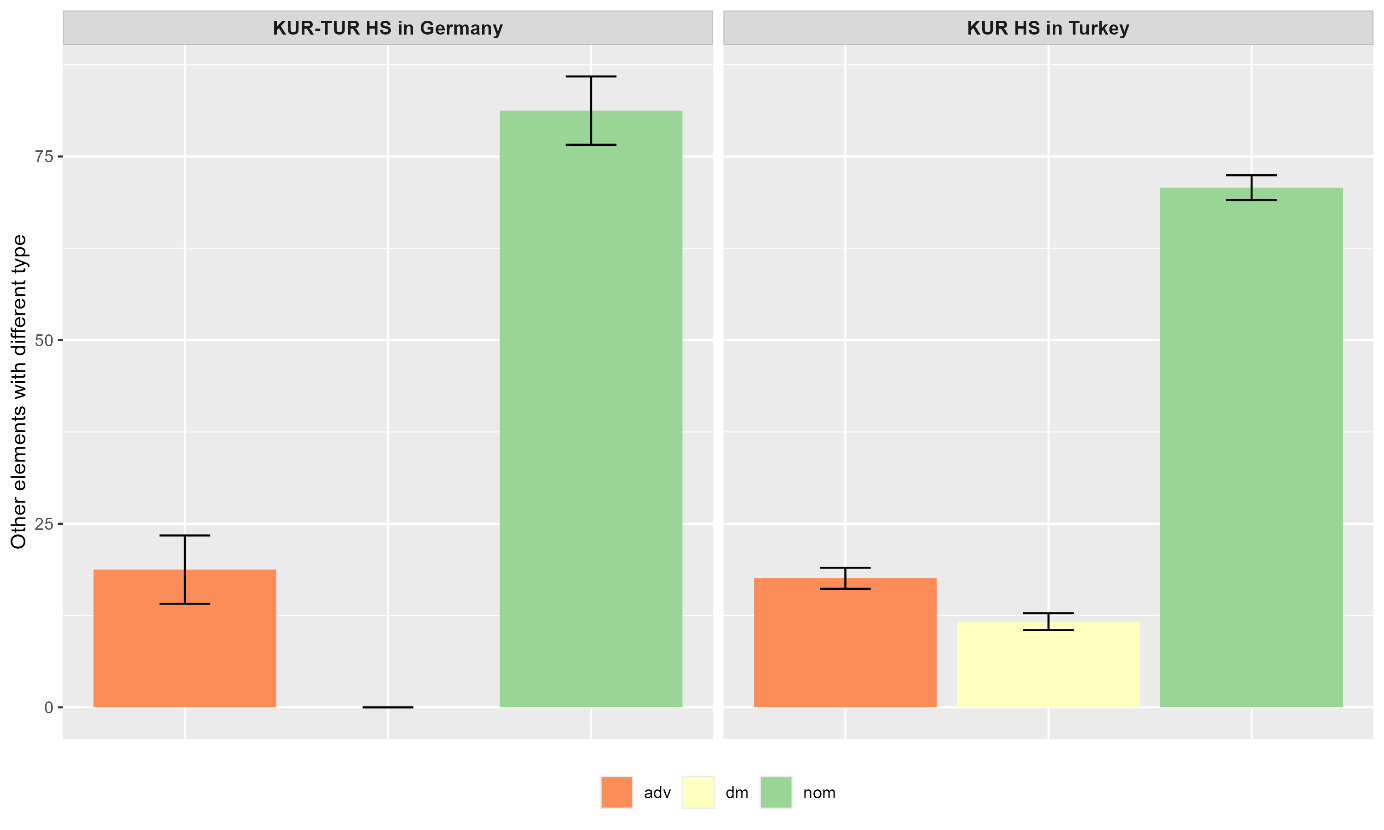
\includegraphics[width=\textwidth]{figures/iefremenko-img023.png}
\caption{\label{fig:key:25}Frequency distribution of non-goal constituents in the post-predicate position (in \%) in relation to the total number of such constituents.}
\end{figure}

\figref{fig:key:25} illustrates the frequency distribution of different types of non-goal constituents in the post-predicate position, expressed as a percentage of the total number of such constituents. The data reveals that, in both groups, non-goal constituents in the post-predicate position predominantly consist of nominal constituents. Specifically, in the data from Turkey, nominal constituents account for over 70\% (n=35) of all non-goal constituents in this position. The percentage of nominal constituents in the post-predicate position in the data from Germany is even higher, exceeding 80\% (n=13).

In addition to nominal constituents, adverbs and discourse markers also appear in the post-predicate position. Adverbs are present in both groups and are used with roughly similar frequency. Notably, Kurmanji speakers in Turkey also use discourse markers in the post-predicate position, which constitute approximately 11\% (seven examples) of the total number of non-goal elements in that context.

Overall, the analysis of the types of non-goal post-predicate elements indicates that both groups predominantly place nominal constituents in this position. While the group in Germany primarily uses nominal constituents (with 13 out of 15 examples being nominal), speakers in Turkey also incorporate adverbs and discourse markers in the post-predicate position. This distribution of non-goal elements may suggest a potential influence from the majority language on Kurmanji: in German, nominal constituents are frequently found in the post-field, while Turkish features a combination of nominal constituents, adverbs, and discourse markers in the post-predicate position, as discussed in \sectref{sec:key:5.3.2}.

\subsubsection{Semantic roles of non-goal nominal constituents in Kurmanji}\label{sec:key:6.3.6.3}

The analysis of types shows that nominal constituents are the most frequent non-goal elements in the post-predicate position. Therefore, the following section will take a closer look at their semantic roles within sentences. To this end, it will distinguish between the following types of semantic roles relevant to the data:

\begin{itemize}
\item cause


\ea \label{ex:key:88} Kurmanji, TUbi05MK\_fwK \\
\gll Şofêr-ê   erebe   pêş-iyê   li   polîs   geriya\\
driver-\textsc{ez}  car  front-\textsc{obl}  in  police  search\textsc{.pst.3sg}\\
\gll \textit{ji bo}     \textit{vî}   \textit{buyer-ê} \\
because-of  this  accident-\textsc{obl}\\
\glt ‘The driver of the front car called the police because of this incident.’ 
  \z


\item comitative (abbreviated as \textit{com} in \figref{fig:key:26}) is a person/thing that accompanies another person/thing in some action


\ea \label{ex:key:89} Kurmanji, DEtr10FK\_iwK \\
\gll Çink-ek   hawo     \textit{ba}   \textit{guddik}, \textit{ba}   \textit{torb-ok}   \textit{sew}\\
woman\textsc{-indf}  have\textsc{.pst.3sg}  with  dog   with  bag-\textsc{indf}  apple\\
‘There was a woman with a dog, with a bag of apples.’ 
  \z


\item location (abbreviated as \textit{loc} in \figref{fig:key:26} below)

\ea \label{ex:key:90} Kurmanji,  TUbi08MK\_iwK \\
\gll Qeza-yek     çêbû       hindik     manû jin-ek     bi-mîn-e   \textit{bin}   \textit{erebê}   \textit{de}\\
accident-\textsc{indf}    happen\textsc{.pst.3sg}  few    leave\textsc{.pst.3sg} woman-\textsc{indf}  \textsc{subj}-stay-\textsc{3sg}  under  car  \textsc{post}\\
\glt ‘There was an accident, and a woman was almost left under the car.’
  \z


\item source


\ea \label{ex:key:91} Kurmanji, TUbi02FK\_isK \\
\gll Ereba   a  sekinî     lê   qewimî     \textit{ji}   \textit{paşde} \\
car  hm  stop\textsc{.pst.3sg}  but  happen\textsc{.pst.3sg}  from  behind\\
\glt ‘The car stopped but bumped from behind.’ 
  \z

\item other – all other categories not mentioned above. I included different roles that occur very rarely in the data, such as possessive for example.
\end{itemize}

\begin{figure}
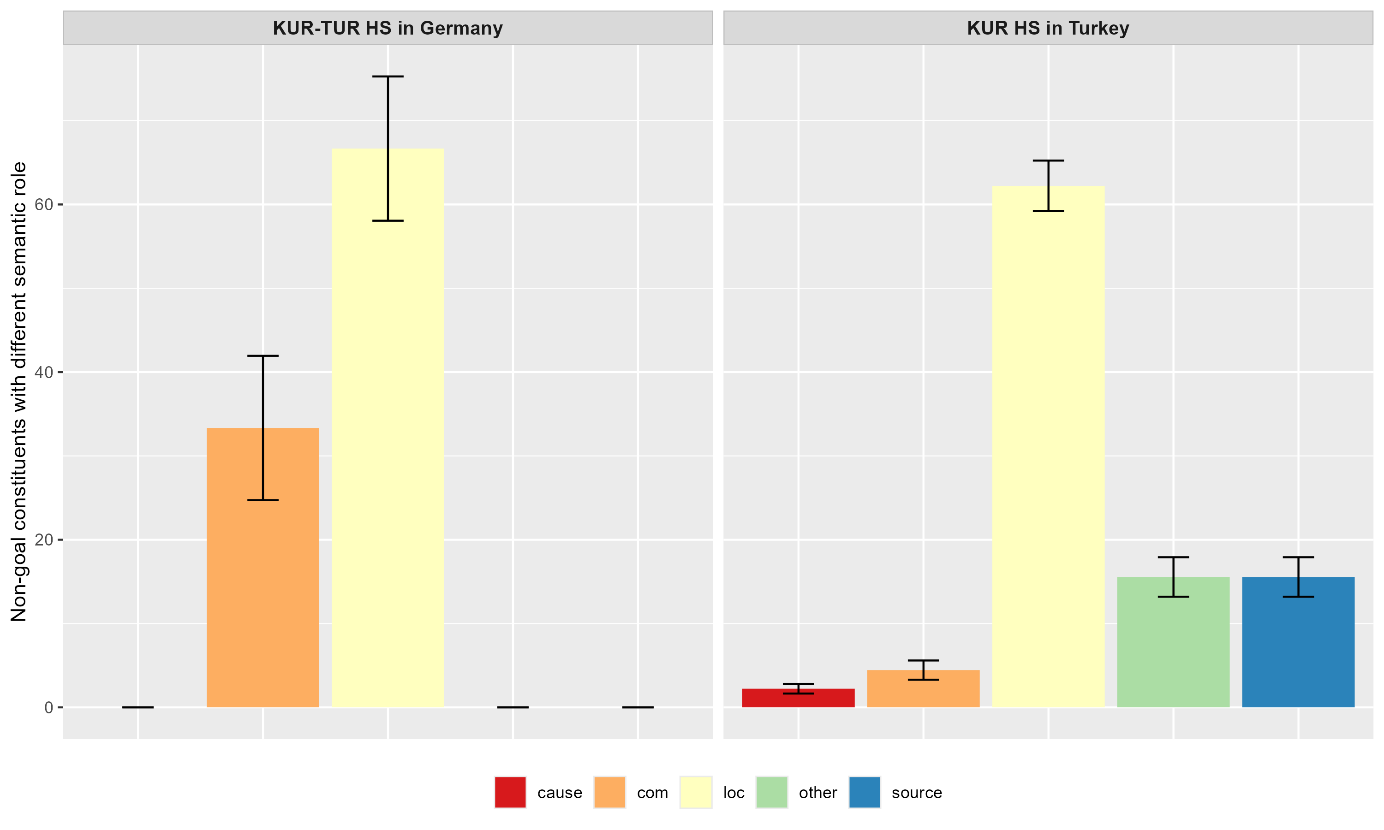
\includegraphics[width=\textwidth]{figures/iefremenko-img024.png}
\caption{\label{fig:key:26}Frequency distribution of semantic roles of non-goal arguments in the post-predicate position (in \%) in relation to the total number of such elements.}

\end{figure}

\figref{fig:key:26} illustrates the frequency of nominal non-goal post-predicate constituents categorized by their specific semantic roles, relative to the total number of nominal non-goal post-predicate constituents. It is important to interpret this distribution with caution due to the low absolute number of nominal structures in the sample.

The data reveal that the most frequently assigned semantic role for non-goal nominal constituents in the post-predicate position is location, which accounts for more than half of all examples in both groups. Additionally, in Germany, participants include constituents with a comitative role in the post-predicate position, while in Turkey, non-goal constituents are assigned various roles, including source, cause/reason, comitative, and others. The broader range of semantic roles observed in Turkey may be attributed to the larger data sample available.

Overall, the analysis of semantic roles does not reveal any significant differences between the groups. Although the absolute number of examples is low, particularly in the German data, the trends across both groups are similar. When speakers in Turkey and Germany place non-goal constituents in the post-predicate position, these constituents primarily denote locations.

\subsubsection{The use of non-goal post-predicate constituents across communicative situations}\label{sec:key:6.3.6.4}

Previous research (\citealt{Haig2014, Haig2018, Gundogdu2019}) suggests that word order in Kurmanji is influenced by predicate semantics, implying that it should not be affected by communicative situations. However, this assertion primarily pertains to goal arguments. Additionally, as mentioned in \sectref{sec:key:3.3.4}, \citet{Frommer1981} and \citet{Haig_post-predicate_EtAl2024-1} found that formality in Persian leads to an increased use of post-predicate structures. Therefore, the following discussion will explore whether formality or mode impacts the use of non-goal constituents in the post-predicate position in Kurmanji.

\begin{figure}
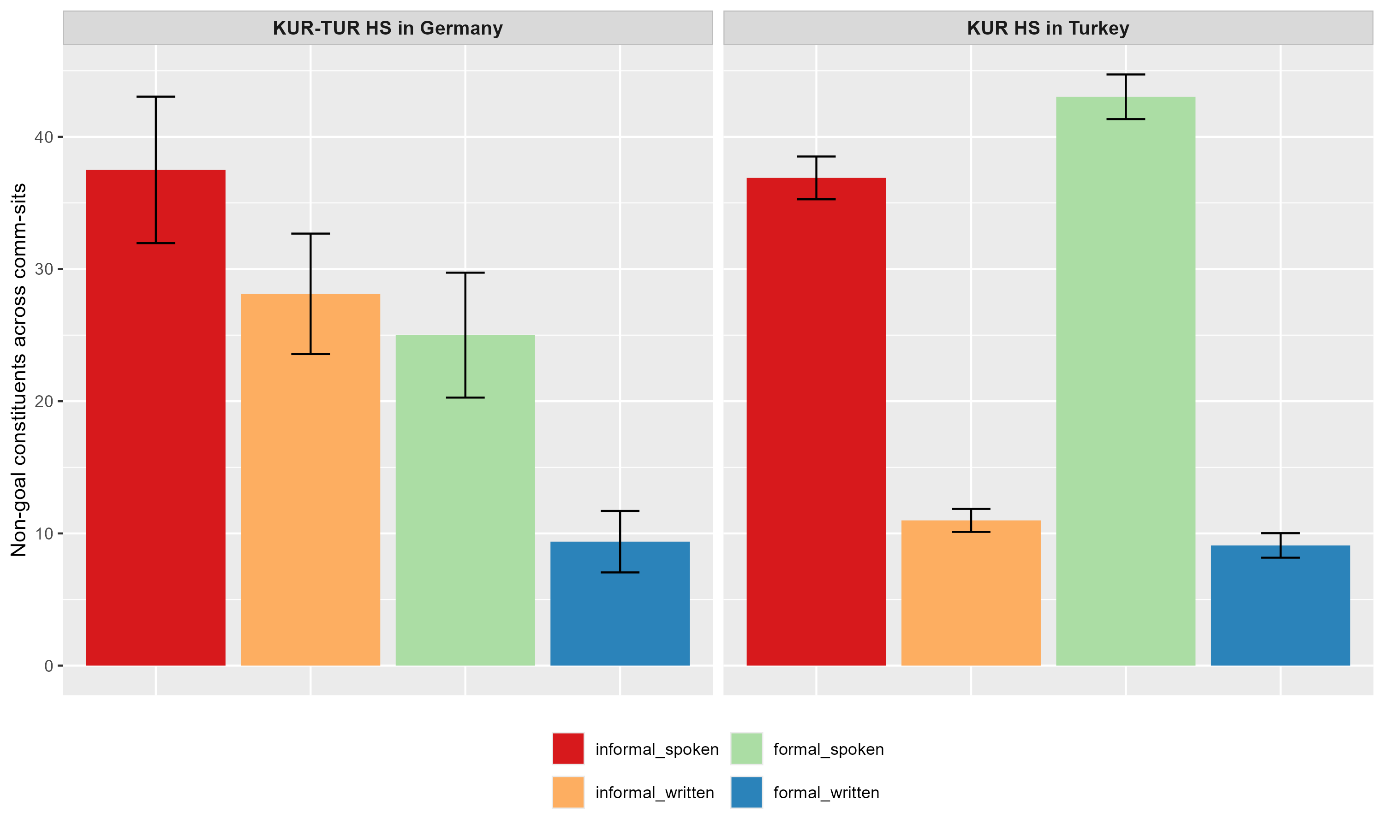
\includegraphics[width=\textwidth]{figures/iefremenko-img025.png}
\caption{\label{fig:key:27}Frequency distribution of non-goal constituents in the post-predicate position (in \%) across different communicative situations in relation to the total number of non-goal constituents.}
\end{figure}

\figref{fig:key:27} illustrates the frequency distribution of non-goal constituents in the post-predicate position relative to the total number of non-goal constituents, with error bars indicating the standard error. The data reveal that both groups use non-goal constituents across the four communicative situations. Notably, for the group in Turkey, the placement of non-goal constituents appears to be more characteristic of the spoken mode, while in Germany, informality seems to be a key predictor for the use of non-goal elements in the post-predicate position.

In summary, the qualitative analysis of non-goal constituents in the post-predicate position indicates that speakers from both groups employ constituents consisting of one or two phonological words. These non-goal elements are predominantly nominal constituents that denote location. Furthermore, the spoken mode appears to positively influence the use of non-goal constituents in the post-predicate position in Turkey, whereas informality seems to affect their placement in Germany. However, it is important to note that these observations are based on a limited number of non-goal constituents.

\section{Summary of the findings}\label{sec:key:6.4}

The current section addresses the findings on word order variation in Kurmanji varieties, specifically focusing on the post-predicate domain. As mentioned at the beginning of this chapter, Kurmanji differs from the heritage languages commonly examined in heritage language research, as it lacks a monolingual variety and does not serve as the societal majority language. Consequently, Kurmanji speakers in both Turkey and Germany are not exposed to the range of registers found in other languages. Therefore, unlike Turkish, not all factors can be analyzed within the context of Kurmanji. This discussion will focus on: \REF{ex:key:1} different language contact situations, including the various contact languages and their intensity of contact, and \REF{ex:key:2} the role of register.

First, the impact of the contact languages on Kurmanji is examined, considering the different intensity of contact between Kurmanji and Turkish compared to Kurmanji and German. The analysis begins with a quantitative analysis of post-predicate structures, revealing that Kurmanji predominantly follows a verb-final word order. On average 23.3 CUs in Germany contain a post-predicate element, compared to 14.9 CUs in Turkey. This finding aligns with previous studies on Kurmanji word order (\citealt{Haig2014}, \citealt{HaigThiele2014, Gundogdu2019}, \citealt{HaigEtAl2024}), which indicate that Kurmanji is predominantly a verb-final language.

At the same time, the data show that speakers in Germany use post-predicate structures more frequently than those in Turkey, with the analysis confirming a significant difference between the groups. However, a closer examination of the types of post-predicate constituents reveals that this increase in Germany is primarily due to a higher number of goals of motion placed in the post-predicate position. Since this position is the default for goal constituents in Kurmanji, the higher frequency of post-predicate structures in Germany may simply reflect a greater expression of motion rather than an influence from contact with German.

Next, the chapter examines the findings with a focus on the different types of constituents employed in the post-predicate position. As demonstrated in Chapter 2, Kurmanji permits three types of goals in the post-predicate position: goals of motion, addressees of verbs of speech, and recipients of verbs of transfer (\citealt{Haig2014, Gundogdu2019}). However, only the first two types appear in the dataset. This is due to the data collection method, as the video shown to participants featured a lot of movement, little interaction and practically no transfer.

An important factor influencing the position of goals in relation to the verb is the type of flagging (\citealt{Haig2014}, \citealt{HaigThiele2014, Gundogdu2019}). Goals marked with the oblique case must be placed in the post-predicate position, whereas the position of those flagged with an adposition is flexible. The only exception is locational nouns, which consistently appear in the post-predicate position because they are derived from nouns \citep{Haig2014}. Moreover, regional variation influences both the position and the types of adpositions used in Kurmanji (\citealt{Haig2014}, \citealt{Haig2022}).

The analysis of the two types of goals that occur in the data showed different results. On the one hand, the position of addressees in the data is in line with the previous research: case-flagged goals are placed in the post-predicate position and goals flagged with the help of adpositions are used in the immediate pre-predicate position. On the other hand, the analysis of goals of motion revealed that sometimes goal arguments are placed noncanonically. While case-flagged goal arguments predominantly occur in the post-predicate position, the data also reveal instances of case-flagged goals appearing in the immediate pre-predicate position.

It is important to highlight that all case-flagged goals of motion appearing in the pre-predicate position in the data from Turkey occur within the same construction, \textit{erdê ketin} (‘to fall on the ground’), where the goal argument \textit{erdê} (‘on the ground’) is placed in the noncanonical pre-predicate position. In Turkish, the contact language, \textit{erdê ketin} corresponds to \textit{yere düşmek}, a fixed construction in which the argument \textit{yere} (‘on the ground’) is consistently positioned before the verb rather than in the post-predicate position.

This pattern is further supported by mono- and bilingual Turkish data from the RUEG sub-corpora (\citealt{LudelingEtAl2024}, \citealt{IefremenkoEtAl2024}), where all instances of \textit{yere} in \textit{yere düşmek} appear before the predicate. Consequently, the noncanonical placement of \textit{erdê} in \textit{erdê ketin} may result from copying of the specific Turkish pattern \textit{yere düşmek}. Alternatively, it may stem from copying of a partially schematic pattern [N-DAT \textit{düşmek}] or a fully schematic pattern [N-DAT V] into Kurmanji.

Aside from the contact-induced explanation, the noncanonical pre-predicate position of the goal argument in \textit{erdê ketin} may also be influenced by the verb itself. In Kurmanji, \textit{ketin} appears in constructions where it functions as a light verb, losing its full lexical meaning, as seen in \textit{bi rê ketin} (‘to set off on a journey’) and \textit{li ber ketin} (‘to meet/encounter’). This could account for the higher frequency of construction copying involving \textit{ketin}, particularly when accompanied by word order changes.

As for the data from Germany, only two instances of case-flagged goal arguments appearing in the immediate pre-predicate position were observed, and neither occurred with the verb \textit{ketin}. Unlike the construction \textit{erdê ketin}, there is no clear evidence that the two noncanonically placed constructions in the German dataset—\textit{pêşiyê bazda} (‘ran ahead’) and \textit{ereba pêşiyê xist} (‘hit the front car’)—were directly copied from German.

The noncanonical placement of these arguments may be attributed to the language acquisition process among Kurmanji heritage speakers in Germany. Their parents’ Kurmanji may have already undergone structural changes due to the contact with Turkish, making these constructions part of the linguistic input provided to the next generation. Additionally, the extension of noncanonical placement to a broader range of constructions may have been reinforced by contact with German. However, drawing definitive conclusions about Kurmanji in Germany remains challenging, as the data come from only nine speakers, and the number of case-flagged goals of motion occurring preverbally is limited to just two examples.

Regarding goals marked with adpositions, previous research on Kurmanji word order indicates that their position is generally flexible, except for locational goals, which are typically restricted to the post-predicate position, similar to case-flagged goals. However, the analysis of the current data revealed instances of goals flagged with locational nouns appearing in the pre-predicate position. Notably, this noncanonical placement occurs in four examples within the Turkish dataset, three of which are used in the construction \textit{hemberî rê} (‘across the road’) with the verbs \textit{revîn} (‘to run’) and \textit{çûn} (‘to go’).

In this context, there is no direct evidence of copying a specific construction for several reasons. First, the construction \textit{hemberî rê} can be used with various verbs. Second, Turkish lacks prepositions, the equivalent construction would be rendered as \textit{yolun karşısına koşmak/gitmek}, where the spatial noun \textit{karşı} (‘opposite’) follows the noun \textit{yol} (‘road’). This suggests that the preverbal position of goal arguments flagged by locational nouns in Kurmanji may result from copying of the schematic [N-DAT V] pattern from Turkish. The findings related to CLI will be revisited in \sectref{sec:key:7.1}.

In the data from Germany, there is only one example of noncanonical argument placement flagged with a locational noun. Similar to the observations regarding case-flagged goals, this noncanonical placement differs from those found in Turkey. Notably, the construction with a preverbal goal argument was produced by the same speaker who also placed a case-flagged goal of motion in the pre-predicate position. As a result, the pre-predicate placement of goals flagged with a locational noun appears to be a characteristic specific to this individual, although it is not the only strategy employed by the speaker.

The usage-based approach underscores the significance of individual speakers in language change (\citealt{Bybee2006}, \citealt{Ansaldo2009}, \citealt{Matras2020}), suggesting that language change arises from the cumulative effects of choices made by individual speakers during their interactions. This finding therefore highlights the importance of examining individual variation, as it allows us to determine whether an innovative construction reflects an idiosyncratic preference of a single speaker or has already begun to propagate across speakers within the community. Distinguishing between these levels of variation is crucial for understanding the dynamics of change in contact settings.

Regarding the other types of adpositions, including prepositions, postpositions, circumpositions, and prepositions combined with locational nouns, the data confirm their flexible positioning. The analysis of the information status of goal arguments did not reveal a correlation between information status and the placement of adpositional goal arguments. However, the form of an adposition appears to influence its position. For instance, there is a tendency for the preposition \textit{bo} (‘to’) to be used in the post-predicate position, while \textit{li} (‘in’) is more commonly placed in the pre-predicate position.

Next, the discussion continues by examining the role of communicative situations in the employment of the post-predicate position in Kurmanji. Previous research (\citealt{Frommer1981}, \citealt{Haig_post-predicate_EtAl2024-1}) indicates a correlation between formality and mode in the use of the post-predicate position in Persian, a language that exhibits characteristics similar to other West Iranian languages. This finding for Persian suggests a possibly similar trend in Kurmanji.

Furthermore, the contact with Turkish and German may lead to the tendency of bi- and trilingual speakers to employ more post-predicate structures in the informal situations and spoken mode. However, the analysis of the frequency distribution of all post-predicate structures across the four communicative situations did not reveal any significant effect of formality or mode on the use of post-predicate structures among either group of Kurmanji speakers. Consequently, no similar developments to those observed in Turkish, German, or Persian were found.

This absence of correlation may stem from the fact that the post-predicate position in the data is primarily used for goal arguments, particularly those flagged with case, which have a fixed position and are thus less sensitive to communicative contexts. Furthermore, it is important to consider that Kurmanji is predominantly used in informal settings, and speakers do not have significant exposure to formal registers in this language.

Interestingly, in the analysis of the placement of adpositional goals of motion in Kurmanji—typically described as flexible in the literature—informality emerged as a significant factor influencing their placement. The regression analysis revealed a tendency for goals of motion flagged with an adposition to be placed in the post-predicate position in the informal situations. This correlation between formality and position may indicate developments similar to those observed in Persian (\citealt{Frommer1981}, \citealt{Haig_post-predicate_EtAl2024-1}) and could also be influenced by contact with Turkish, where the post-predicate position is common in informal situations. The role of register will be addressed in \sectref{sec:key:7.3}.

Moreover, the analysis of post-predicate constituents in Kurmanji revealed the presence of non-goal constituents in this position, with their usage being facilitated by the spoken mode among Kurmanji speakers in Turkey. This tendency can be attributed to the spontaneous nature of spoken speech, which is inherently more open to word order variation compared to the written mode, where there is more time for corrections and editing. If the spoken mode leads to an increased use of non-goal post-predicate structures in Kurmanji, a similar pattern would be expected in the data from Germany. However, the analysis of the placement of non-goal constituents across different communicative situations in Germany did not demonstrate any effect of mode. It is important to note, though, that the limited number of examples of non-goal constituents, particularly in the German data, makes it challenging to draw definitive conclusions regarding their frequency distribution across various communicative situations.

In summary, the analysis of post-predicate constituents in Kurmanji reveals that word order in both Germany and Turkey is strongly influenced by predicate semantics. The majority of post-predicate constituents consist of goals of motion and addressees of verbs of speech. While the placement of addressees is consistent with previous research, there are noncanonical examples for goals of motion. Specifically, goals flagged with case or locational nouns also occupy the pre-predicate position, particularly in certain constructions within the Turkish data. Similarly, preverbal case-flagged goal arguments and those flagged with locational nouns are found in the German data, though they appear in various constructions. Lastly, the analysis indicates that the placement of adpositional goals is flexible, with informal registers leading to the use of the post-predicate position. While non-goal constituents do occur in the post-predicate position, their frequency is low, and their usage is mainly associated with the spoken mode of Kurmanji in Turkey. This spoken mode is characterized by spontaneity and a greater openness to word order variation.

